\documentclass{article}

\usepackage{arxiv}

\usepackage[utf8]{inputenc} % allow utf-8 input
\usepackage[T1]{fontenc}    % use 8-bit T1 fonts
\usepackage{lmodern}        % https://github.com/rstudio/rticles/issues/343
\usepackage{hyperref}       % hyperlinks
\usepackage{url}            % simple URL typesetting
\usepackage{booktabs}       % professional-quality tables
\usepackage{amsfonts}       % blackboard math symbols
\usepackage{nicefrac}       % compact symbols for 1/2, etc.
\usepackage{microtype}      % microtypography
\usepackage{graphicx}

\title{Seabird assemblages are linked to the major western boundary current off eastern Australia}

\author{
    Nicholas W. Daudt*
   \\
    Department of Marine Science \\
    University of Otago \\
  Dunedin, Aotearoa New Zealand \\
  \texttt{\href{mailto:nicholaswdaudt@gmail.com}{\nolinkurl{nicholaswdaudt@gmail.com}}} \\
   \And
    Eric J. Woehler
   \\
    Australasian Seabird Group \\
    BirdLife Australia \\
  Hobart, Australia \\
  \texttt{\href{mailto:eric.woehler@gmail.com}{\nolinkurl{eric.woehler@gmail.com}}} \\
   \And
    Matthew R. Schofield
   \\
    Department of Mathematics and Statistics \\
    University of Otago \\
  Dunedin, Aotearoa New Zealand \\
  \texttt{\href{mailto:matthew.schofield@otago.ac.nz}{\nolinkurl{matthew.schofield@otago.ac.nz}}} \\
   \And
    Robert O. Smith
   \\
    Department of Marine Science \\
    University of Otago \\
  Dunedin, Aotearoa New Zealand \\
  \texttt{\href{mailto:robert.smith@otago.ac.nz}{\nolinkurl{robert.smith@otago.ac.nz}}} \\
   \And
    Leandro Bugoni
   \\
    Institute of Biological Sciences \\
    Universidade Federal do Rio Grande--FURG \\
  Rio Grande, RS, Brazil \\
  \texttt{\href{mailto:lbugoni@yahoo.com.br}{\nolinkurl{lbugoni@yahoo.com.br}}} \\
   \And
    William J. Rayment
   \\
    Department of Marine Science \\
    University of Otago \\
  Dunedin, Aotearoa New Zealand \\
  \texttt{\href{mailto:will.rayment@otago.ac.nz}{\nolinkurl{will.rayment@otago.ac.nz}}} \\
  }


% tightlist command for lists without linebreak
\providecommand{\tightlist}{%
  \setlength{\itemsep}{0pt}\setlength{\parskip}{0pt}}

% From pandoc table feature
\usepackage{longtable,booktabs,array}
\usepackage{calc} % for calculating minipage widths
% Correct order of tables after \paragraph or \subparagraph
\usepackage{etoolbox}
\makeatletter
\patchcmd\longtable{\par}{\if@noskipsec\mbox{}\fi\par}{}{}
\makeatother
% Allow footnotes in longtable head/foot
\IfFileExists{footnotehyper.sty}{\usepackage{footnotehyper}}{\usepackage{footnote}}
\makesavenoteenv{longtable}

% Pandoc citation processing
\newlength{\cslhangindent}
\setlength{\cslhangindent}{1.5em}
\newlength{\csllabelwidth}
\setlength{\csllabelwidth}{3em}
\newlength{\cslentryspacingunit} % times entry-spacing
\setlength{\cslentryspacingunit}{\parskip}
% for Pandoc 2.8 to 2.10.1
\newenvironment{cslreferences}%
  {}%
  {\par}
% For Pandoc 2.11+
\newenvironment{CSLReferences}[2] % #1 hanging-ident, #2 entry spacing
 {% don't indent paragraphs
  \setlength{\parindent}{0pt}
  % turn on hanging indent if param 1 is 1
  \ifodd #1
  \let\oldpar\par
  \def\par{\hangindent=\cslhangindent\oldpar}
  \fi
  % set entry spacing
  \setlength{\parskip}{#2\cslentryspacingunit}
 }%
 {}
\usepackage{calc}
\newcommand{\CSLBlock}[1]{#1\hfill\break}
\newcommand{\CSLLeftMargin}[1]{\parbox[t]{\csllabelwidth}{#1}}
\newcommand{\CSLRightInline}[1]{\parbox[t]{\linewidth - \csllabelwidth}{#1}\break}
\newcommand{\CSLIndent}[1]{\hspace{\cslhangindent}#1}

\usepackage{setspace}\doublespacing
\usepackage[left]{lineno}
\newcommand{\blinenumbers}{\begin{linenumbers}}
\newcommand{\elinenumbers}{\end{linenumbers}}
\usepackage{pdflscape}
\DeclareUnicodeCharacter{0394}{\ensuremath{\Delta}}
\newcommand{\blandscape}{\begin{landscape}}
\newcommand{\elandscape}{\end{landscape}}
\usepackage{booktabs}
\usepackage{longtable}
\usepackage{array}
\usepackage{multirow}
\usepackage{wrapfig}
\usepackage{float}
\usepackage{colortbl}
\usepackage{pdflscape}
\usepackage{tabu}
\usepackage{threeparttable}
\usepackage{threeparttablex}
\usepackage[normalem]{ulem}
\usepackage{makecell}
\usepackage{xcolor}
\begin{document}
\maketitle


\begin{abstract}
\textbf{Aim:} To identify assemblages of seabird species and relate them to environmental conditions off eastern Australia, a world seabird hotspot.
\textbf{Location:} East coast of Australia.
\textbf{Methods:} We used 15 seabird at-sea ship-based survey data sets collected over 37° of latitude, from 2016 to 2021, and fitted Region of Common Profile (RCP) mixture models for each season and type of data (presence-absence and abundance). RCP groups are defined as a set of regions where the probability of encountering a specific species profile is constant within regions, but different amongst them. These groups also vary according to covariates, which in our case included oceanographic, climatic, and physiographic parameters.
\textbf{Results:} Based on 142,646 seabirds recorded, from 80 species, all models suggested two macro-scale assemblages (`northern' and `southern'), except for the autumn presence-absence model that identified three groups. The model results consistently show a biogeographic transition at \textasciitilde34°S, near the latitude at which the East Australian Current separates from the Australian continental slope. Sea surface temperatures or sea surface salinities were selected in all final models, further indicating a close relationship between seabird assemblages and water masses. Results from both data types, presence-absence and abundance, resulted in similar spatial and species profile patterns.
\textbf{Main conclusions:} RCP models clearly identified two seabird assemblages off the east coast of Australia, suggesting the persistence of these groups at seasonal and macro spatial scales. Given the rapid climatic changes that the East Australian Current is experiencing and its importance in influencing distributions of seabirds, the methods applied in our study could be replicated to assess possible changes in seabird assemblages, and how they are affected by changing environmental conditions.
\end{abstract}

\keywords{
    Assemblages
   \and
    Biogeography
   \and
    Community ecology
   \and
    East Australian Current
   \and
    Mixture models
   \and
    Region of Common Profiles
  }

\hypertarget{orcid}{%
\section*{ORCID}\label{orcid}}
\addcontentsline{toc}{section}{ORCID}

Nicholas W. Daudt \url{https://orcid.org/0000-0001-8211-8771}

Eric J. Woehler \url{https://orcid.org/0000-0002-1125-0748}

Matthew R. Schofield \url{https://orcid.org/0000-0003-1481-2766}

Robert O. Smith \url{https://orcid.org/0000-0001-5931-3843}

Leandro Bugoni \url{https://orcid.org/0000-0003-0689-7026}

William J. Rayment -- \url{https://orcid.org/0000-0001-9558-5109}

\hypertarget{biosketch}{%
\section*{Biosketch}\label{biosketch}}
\addcontentsline{toc}{section}{Biosketch}

\textbf{Nicholas W. Daudt (he/him)} is broadly interested in spatial ecology and ecological modelling. His research uses data science and modelling to understand biogeographic patterns and ecological processes that build marine top predators' biodiversity patterns across space and time.

\hypertarget{acknowledgements}{%
\section*{Acknowledgements}\label{acknowledgements}}
\addcontentsline{toc}{section}{Acknowledgements}

We thank all observers who assisted in data collection, the crews of RV \emph{Investigator} and RV \emph{Falkor}, and the Australasian Seabird Group (BirdLife Australia) for logistical support. The authors would like to thank Dr.~Skipton N.C. Woolley, \texttt{\{ecomix\}} developer, who kindly helped NWD build preliminary models and gave advice in several stages of model construction. NWD is supported by a Doctoral scholarship from the University of Otago.

\begin{center}\rule{0.5\linewidth}{0.5pt}\end{center}

\textbf{Data availability statement:} The gridded data used as the basis for all analyses are available in the archived repository along with the code to reproduce the results. The raw data are currently being used for other projects and thus can not be publicly available. If you are interested in the raw data, please get in touch with Eric J. Woehler.

\textbf{Funding statement:} Parks Australia provided funding support to participants for selected voyages.

\textbf{Conflict of interest disclosure:} The authors declare no conflict of interest.

\textbf{Ethics approval statement:} NA.

\textbf{Patient consent statement:} NA.

\textbf{Permission to reproduce material from other sources:} NA.

\textbf{Clinical trial registration:} NA.

\newpage

\begin{linenumbers}

\begin{center}
\textbf{Seabird assemblages are linked to the major western boundary current off eastern Australia}
\end{center}

\emph{Running title:} Seabird assemblages off Eastern Australia

\begin{center}\rule{0.5\linewidth}{0.5pt}\end{center}

\textbf{Abstract}

\textbf{Aim:} To identify assemblages of seabird species and relate them to environmental conditions off eastern Australia, a world seabird hotspot.

\textbf{Location:} East coast of Australia.

\textbf{Methods:} We used 15 seabird at-sea ship-based survey data sets collected over 37° of latitude, from 2016 to 2021, and fitted Region of Common Profile (RCP) mixture models for each season and type of data (presence-absence and abundance). RCP groups are defined as a set of regions where the probability of encountering a specific species profile is constant within regions, but different amongst them. These groups also vary according to covariates, which in our case included oceanographic, climatic, and physiographic parameters.

\textbf{Results:} Based on 142,646 seabirds recorded, from 80 species, all models suggested two macro-scale assemblages (`northern' and `southern'), except for the autumn presence-absence model that identified three groups. The model results consistently show a biogeographic transition at \textasciitilde34°S, near the latitude at which the East Australian Current separates from the Australian continental slope. Sea surface temperatures or sea surface salinities were selected in all final models, further indicating a close relationship between seabird assemblages and water masses. Results from both data types, presence-absence and abundance, resulted in similar spatial and species profile patterns.

\textbf{Main conclusions:} RCP models clearly identified two seabird assemblages off the east coast of Australia, suggesting the persistence of these groups at seasonal and macro spatial scales. Given the rapid climatic changes that the East Australian Current is experiencing and its importance in influencing distributions of seabirds, the methods applied in our study could be replicated to assess possible changes in seabird assemblages, and how they are affected by changing environmental conditions.

\textbf{\emph{Keywords}} Assemblages; Biogeography; Community ecology; East Australian Current; Mixture models; Region of Common Profiles

\newpage

\hypertarget{introduction}{%
\section{Introduction}\label{introduction}}

Bioregionalization is the discipline that identifies, delimits, characterises, and names biogeographical regions (Morrone, 2018; Vilhena \& Antonelli, 2015). Although there is often no agreement on the naming systems among proposed regionalization schema (but see Ebach et al., 2008), the hierarchical nature of bioregions is well recognized (Kreft \& Jetz, 2010; Vilhena \& Antonelli, 2015). Thus, bioregions are usually described within geographically larger classifications, such as `provinces' or `realms' (Costello et al., 2017; Spalding et al., 2007). The delimitation of bioregions is made through identifying sets of species that are endemic or have high levels of co-occurrence, and are distinct enough from other regions. In this sense, bioregions are interpreted as natural representations of common historical and/or ecological processes shaped by physical and biological forces (Kreft \& Jetz, 2010). In particular, the identification of bioregions allows representation of the distribution of multiple species at a given time and space, and relating these regions to environmental characteristics. By doing so, bioregions can be interpreted as species assemblages (N. A. Hill et al., 2017; Lyons et al., 2017). Given these features, bioregions can be used as surrogates for biodiversity monitoring in data-poor regions and in regional conservation planning (Ferrier, 2002; Spalding et al., 2007), playing a fundamental role in conservation biogeography (Whittaker et al., 2005).

Seabird assemblages have been widely described and related to environmental characteristics (Hyrenbach et al., 2007; Ribic et al., 1997; Woehler et al., 2003). Considering the hierarchical nature of oceanographic processes and their resulting features (Haury et al., 1978), it is not surprising that the distribution of highly mobile seabirds are linked differently across temporal and spatial scales (Haury et al., 1978; Hunt \& Schneider, 1987). In the marine environment, large scale (\textgreater100 km length) oceanographic features (e.g.~boundary currents and water masses) act as terrestrial biomes (based on vegetation), and influence seabird assemblage structure--i.e.~the occurrence of species and their relative numerical composition (Commins et al., 2014; Hyrenbach et al., 2007; Ribic et al., 1997). In contrast, local abundance is related to meso- (10--100 km) and sub-mesoscale (1--10 km) processes that aggregate prey and therefore predators, such as fronts and eddies (Scales, Miller, Hawkes, et al., 2014; Weimerskirch, 2007). Such processes, although relatively ephemeral, are primarily driven by physical and atmospheric forces, and are thus somewhat predictable in space and time, providing consistent feeding areas for marine predators when they occur (Davoren, 2013; Hazen, Suryan, et al., 2013). Sea surface temperatures are a key driver of seabird distributions, at individual- and assemblage-levels, operating over a range of spatial and temporal scales from macro (e.g.~water masses) to fine (e.g.~fronts) (Dunlop et al., 1988; Quillfeldt et al., 2015; Ribic et al., 1997). Despite extensive surveys (e.g. Ballance et al., 1997) and tracking studies (e.g. Carneiro et al., 2020), many oceanic regions still lack information on the distributions and abundances of seabird species, and how they assemble in space and time.

One area in need of better understanding of seabird distributions is Australia, considered a global seabird hotspot (Karpouzi et al., 2007; Ramírez et al., 2017). Given the region's importance for seabird diversity, there are surprisingly few studies on seabird distributions at sea (Bernard et al., 2021; Mott \& Clarke, 2018). Off northwest Australia, at-sea surveys, multivariate analyses (Dunlop et al., 1988) and ensemble species distribution models of species assemblages (Lavers et al., 2014) showed that habitat use by tropical seabird species was related to sea surface temperatures and salinity. Dunlop et al. (1988) suggested that salinity was the main variable influencing species' distributions in oceanic waters while temperature was the key factor for species on the continental shelf. In contrast, there are few studies at large spatial and temporal scales off eastern Australia. T. A. Reid \& Hindell (2000) and Evans et al. (2021) analysed seabird assemblages and their relationships with oceanographic and prey data at mesoscale off southeast Tasmania. The remaining studies are mostly descriptive accounts locally (Blaber \& Milton, 1994; Norman, 1992), or focused on a single species (Priddel et al., 2014).

The East Australian Current (EAC) is the major western boundary current in the South Pacific Ocean, and the dominant boundary current off eastern Australia (Ganachaud et al., 2014). The EAC has been extensively studied, although the links between the EAC's oceanography and marine predators are not well known. The dynamic features associated with the EAC, such as mesoscale eddies and upwelling, are likely to influence marine biota (Scales, Miller, Hawkes, et al., 2014; Suthers et al., 2011). While most of the biological studies in this system were focused on plankton entrapment within the cores of eddies (Firme et al., 2023; Garcia et al., 2022; Hassler et al., 2011), there is a growing body of work focusing on fisheries (Brieva et al., 2015; Hobday, 2010; Young et al., 2011). These studies emphasized how the probability of occurrence of a given taxon, and the structure of species assemblages, were driven by the EAC. However, the relationships between oceanography and marine megafauna within the EAC are poorly known (Suthers et al., 2011). Some progress has been made using shark and ray movement data (Jaine et al., 2014; Niella et al., 2020; Niella et al., 2022), and satellite tracking has also demonstrated that increased sea surface temperatures in the EAC decreases little penguin \emph{Eudyptula minor} foraging success (Carroll et al., 2016), but information at the assemblage-level for seabirds in the EAC is absent.

Marine species range shifts are more likely to occur faster than terrestrial species due to their higher sensitivity to warming (Lenoir et al., 2020; Pinsky et al., 2019). As a result, climate change is rearranging the structure of species assemblages around the globe (Antão et al., 2020; Dornelas et al., 2014; Poloczanska et al., 2013). Top predators, for instance, may change their core habitats (Hazen, Jorgensen, et al., 2013; Reisinger et al., 2022), with unprecedented population consequences (Woehler \& Hobday, 2023). For seabirds, Péron et al. (2010) and Sojitra et al. (2022) showed that sea surface temperature anomalies affected the occurrence and abundances of albatross and petrel species with latitude, thus affecting assemblage structure. In eastern Australia, changing EAC conditions have affected a range of marine species. For example, changes in zooplankton assemblage structure and fish distribution patterns have been recorded and attributed to warming water temperatures, and shifts in shark distributions are expected (C. R. Johnson et al., 2011; Niella et al., 2022). A severe marine heatwave driven by a poleward strengthening of the EAC, showed drastic environmental impacts including disease outbreaks in aquaculture farms and wildlife mortalities (Oliver et al., 2017). Given that the EAC is strengthening and extending farther southward and getting warmer (Cai et al., 2005; Phillips et al., 2022), biological changes are expected to occur (Hobday, 2010; Poloczanska et al., 2007).

In light of eastern Australia's importance for seabirds, and the recent attention on how predicted climate change will influence the EAC's marine biota (Poloczanska et al., 2007), an assessment of the contemporary spatial distributions of seabirds within the EAC at large temporal and spatial scales is timely. Seabirds can serve as sentinels for tracking ecological changes in the EAC in many ways (e.g. Sydeman et al., 2012). Surprisingly though, seabird distribution is under-represented in climate change studies, despite being highlighted as a priority topic (Grémillet \& Boulinier, 2009; Sydeman et al., 2012).

In this study, we aim to identify assemblages of seabird species within the EAC and adjacent areas, and relate these assemblages to environmental conditions, by using at-sea survey data and a state-of-the-art modelling technique. We use the Region of Common Profiles {[}RCP; Foster et al. (2013){]}, a mixture model regarded as one of the best available tools for describing bioregions (N. A. Hill et al., 2020; S. N. C. Woolley et al., 2020). RCP is a model-based approach, and has a range of advantages over traditional algorithm-based statistics (N. A. Hill et al., 2020; Warton et al., 2015). Eastern Australia supports a high diversity of seabirds and offers wide environmental gradients over a near 40° latitudinal range, from the tropics to the cool temperate. We hypothesised to find different seabird assemblages relating to different environmental conditions within the EAC. In addition, presence-absence and abundance data were used to test if the different numerical resolutions would result in the identification of similar assemblages. This study provides a repeatable framework on which future studies can assess how future changes in the EAC may influence the distribution of seabird assemblages.

\hypertarget{methods}{%
\section{Methods}\label{methods}}

\hypertarget{study-area}{%
\subsection{Study area}\label{study-area}}

The EAC originates from the South Equatorial Current (SEC), a tropical nutrient-poor current. When the SEC's North Caledonian Jet meets the Queensland Plateau (\textasciitilde18°S), it splits into a north-flowing branch towards the Gulf of Papua and a south-flowing branch, which marks the start of the EAC (Ganachaud et al., 2014; Kessler \& Cravatte, 2013). The South Caledonian Jet completes the EAC system at \textasciitilde22°S after encountering the shelf break in the southern portion of the Great Barrier Reef (\textbf{Figure \ref{fig:fig1-study-area}a}; Kessler \& Cravatte (2013); Ganachaud et al. (2014)). The EAC interacts with the bathymetry of the seafloor, giving rise to oceanographic features and processes, such as smaller currents, upwellings, and persistent dynamic eddies (Oke, Roughan, et al., 2019; Oke \& Middleton, 2000; Ridgway \& Dunn, 2003). The EAC flows polewards and is primarily associated with the shelf break, but at \textasciitilde32°S it detaches from the shelf and spawns an area of eddy generation that dissipates throughout the western Tasman Sea (Mata et al., 2006; Oke, Roughan, et al., 2019), the `EAC eastern extension' (Oke, Pilo, et al. (2019); often termed the `Tasman Front'). Although most EAC energy is converted into eddies, the EAC still runs southwards following the shelf break towards Tasmania (the `EAC southern extension'; \textbf{Figure \ref{fig:fig1-study-area}a}), carrying eddy-like features as a transient current (Oke, Roughan, et al., 2019).

\hypertarget{seabird-and-environmental-data-sources}{%
\subsection{Seabird and environmental data sources}\label{seabird-and-environmental-data-sources}}

Seabird data were gathered aboard \emph{RV Investigator} and \emph{RV Falkor} on 15 voyages, between 2016/17--2020/21, spanning over \textasciitilde37° of latitude (\textbf{Figure \ref{fig:fig1-study-area}b}; \textbf{Table S1}). One or more observers continuously recorded seabirds within a 300 m forward quadrant (eye height 25 m a.s.l) from sunrise to sunset hours while the ship was underway. The species, the numbers of birds, and their behaviours were logged in real time into a ship-based web server. Environmental parameters for atmospheric and oceanographic conditions were logged continuously by automated-ship based sensors, with seabird observations supplementing relevant environmental conditions such as visibility or associations with marine mammals. Individual records received a date/time/geographic coordinate label (multi-species records have the same label but are logged as separate entries for each species). Birds following the vessels were excluded from analyses. Seabird observation protocols followed Raymond et al. (2010), in use around Australia since 1980.

To investigate and predict species' distributions and relationships with environmental variables, a considered choice of broad-scale climatic and oceanographic covariates is important (Barbet-Massin \& Jetz, 2014). We used three physiographic variables and seven oceanographic variables, from which a further three climatic layers were calculated (\textbf{Table \ref{tab:table1}}). These variables are the most frequently used in seabird-environment relationship studies (Tremblay et al., 2009), capturing processes at a range of spatial and temporal scales from macro-scale water-mass properties to prey availability in meso- to submesoscale oceanographic features (Haury et al., 1978; Scales, Miller, Hawkes, et al., 2014; Weimerskirch, 2007).

\hypertarget{data-treatment}{%
\subsection{Data treatment}\label{data-treatment}}

Data wrangling, modelling and visualization were done in R 4.2.0 (R Core Team, 2022); the full list of packages can be found in the Supplementary Material. Code and the modelling dataset (see \ref{sec:modellingdatasets}) are available in \textbf{(Zenodo repo)}.

\hypertarget{environmental-layers}{%
\subsubsection{Environmental layers}\label{environmental-layers}}

The spatial and temporal persistence of oceanographic features such as eddy kinetic energy (`eke') and thermal fronts (sea surface temperature gradient: `sst\_grad') may influence the movements and distributions of seabirds by offering a higher likelihood of finding food (Scales, Miller, Embling, et al., 2014; Weimerskirch, 2007). Thus, `eke' and `sst\_grad' environmental layers were calculated before extracting environmental data for each seabird record. For both `eke' and `sst\_grad', we used their original cell spatial resolution (\textbf{Table \ref{tab:table1}}) and calculations were done layer-by-layer to match seabird data on the finest spatial scale possible. Eddy kinetic energy was calculated as \(0.5 (u'² + v'²)\), where \(u' = u - \bar{u}\) and \(v' = v - \bar{v}\) are the surface zonal (latitudinal) and meridian (longitudinal) geostrophic currents, respectively, using a rolling mean of 90 days as \(\bar{u}\) and \(\bar{v}\) (Sun et al., 2022). The spatial `sst\_grad' for each cell was calculated by averaging the maximum value for each neighbouring cell (average neighbourhood maximum), from north-to-south (NS) and west-to-east (WE); then, the magnitude of the gradient was defined as \(NS² + WE²\) (Burrows et al., 2011). In addition, we calculated climatic seasonal average layers for `eke' and `sst\_grad' based on the 11-year data for 2011--2021 as a proxy for persistent oceanographic features, and the `eke' standard deviation over the same period (named with the prefix `clim\_' in \textbf{Table \ref{tab:table1}}). Seabed slope was calculated using `raster::terrain()' (Hijmans, 2022a), and distance from the coast was calculated through `sf::st\_distance()' (Pebesma, 2018) using Australia and Tasmania as the mainland (i.e.~ignoring smaller islands). Then, for each seabird record, the most proximate value for each environmental layer (original or calculated) was extracted using built-in functions from `raster' 3.5-21, `terra' 1.6-7, and `sf' 1.0-8 packages (Hijmans, 2022a, 2022b; Pebesma, 2018).

\hypertarget{modellingdatasets}{%
\subsubsection{Data}\label{modellingdatasets}}

\label{sec:modellingdatasets}

Seabirds are highly mobile animals, and many species migrate and/or disperse during their non-breeding periods (Schreiber \& Burger, 2002). Therefore, seasonal differences in species composition were expected (e.g. K. Reid et al., 2023), and in the probabilities of occurrence and in total numbers. Thus, we built separate modelling datasets for each season. We aggregated seabird data by 1° latitude \(\times\) 1° longitude grid cells (\emph{c.} 110 \(\times\) 110 km) and season (\textbf{Figure \ref{fig:fig1-study-area}b}), by summing seabirds from the same species. To test if the presence-absence and abundance (raw counts) data would result in similar assemblage patterns, we built two species matrices, where the presence-absence matrix transformed values \textgreater1 to 1. To avoid numerical instabilities in the models prompted by unusual or rare species, we kept only species occurring in at least six grids within each season (summer = 12 species; autumn = 21; winter = 20; spring = 33). The associated environmental data of each seabird record were averaged within the same grid cells and seasons, and environmental data were standardised before modelling.

\hypertarget{statistical-modelling}{%
\subsection{Statistical modelling}\label{statistical-modelling}}

We used the mixture model Region of Common Profiles (RCP) to identify and describe seabird species assemblages. RCP is a one-stage bioregionalization approach, as it identifies bioregions by specifying a statistical model that simultaneously relates response (multi-species data) and predictor (environmental data) (N. A. Hill et al., 2020; S. N. C. Woolley et al., 2020). Given a set of environmental variables, the model can predict assemblage probabilities for sites where no biotic (observational) data exist. As a model-based approach, RCPs can be compared by information criteria, present uncertainty around the results, and check for model assumptions through assessing distribution of residuals (N. A. Hill et al., 2020; Warton et al., 2015).

The model is specified in terms of assemblages and site-specific probabilities. There are \(K\) assemblages (i.e.~RCPs), \(K = (1, ..., k)\), that are common across the study area. The outcome variable is a vector \(y_{i} = (y_{i1}, ... y_{iS})\), that gives the count or presence-absence of each of the \(S\) species at site \(i\). Depending on whether we model the counts or presence-absence data, the assemblages are defined in terms of the expected frequency or relative frequency of the species, respectively. An output of the model is the estimated probability that site \(i\) has each of the \(K\) possible assemblages. RCPs are a multivariate adaptation of a mixture-of-experts model; as such, the mixing proportions (assemblage structure) vary according to covariates (predictors) (Foster et al., 2013). However, the final estimated assemblage structure is assumed to be constant for all sites belonging to the \(K\) assemblages (Foster et al., 2013). As such, RCPs can be directly interpreted as assemblages, and their species profiles as the assemblage structure.

Before fitting models, covariates were checked for collinearity within each seasonal dataset. If a pairwise collinearity of \(\left|x\right| >0.7\) was found we removed one of the variables (Dormann et al., 2013), favouring direct measures over the `climatic' layers we calculated (e.g.~if `sst\_grad' and `clim\_sst\_grad' were correlated, we chose `sst\_grad'). Thus, `full models' differed between seasons as the retained covariates varied, although most covariates were common for all seasons.

Due to seabird migration and dispersion, seasons could act as `sampling artifacts' (Foster et al., 2017), thus biasing results (Ponti \& Sannolo, 2023). In light of the difference among seasons in the numbers of species that met our occurrence threshold (see \ref{sec:modellingdatasets}), we decided to use RCP models by season and data type (presence-absence and abundance). RCP models were used to relate the response variables (i.e.~presence-absence or abundance of each seabird species in each grid cell) to the independent predictor covariates (i.e.~averaged values of environmental variables in each cell). Presence-absence data were modelled based on a Bernoulli model, whereas abundance data were based on a Negative Binomial model. RCPs were fitted using the `ecomix' 1.0.0 package (S. Woolley et al., 2022), with the following workflow: (i) find the best number of groups (\(K\)) that describes the data, (ii) re-fit the model by fixing \(K\) and selecting the optimal combination of covariates, (iii) check residuals, (iv) bootstrap the best model to estimate uncertainty around parameter estimates, and (v) produce results.

To identify the best number of RCP groups (\(K\)) that described the data, we used full models (all covariates) with 100 random start numbers (see Foster et al., 2013) between \(k = (2, ..., 7)\) groups, and chose the number of RCPs that minimized the Bayesian Information Criterion (BIC). Then, we fixed \(K\) at the optimal number and fitted models for every possible linear, additive combination of covariates. We chose the best model as the one with the lowest BIC. Visual inspection of randomized quantile residual plots modified for mixture models was used to verify model assumptions (Dunstan et al., 2013). To obtain estimates of uncertainty for model parameters (confidence intervals), we used the default settings of `ecomix::regional\_mix.bootstrap()', which applies a Bayesian bootstrap 1000 times. A custom code was written to generate partial plots for exploring the influence of covariates on RCP membership.

We built a seasonal 11-year (2011--2021) average layer for predicting model results for each environmental covariate. These variables were then averaged within 1° latitude \(\times\) 1° longitude grid cells, by season, between 9--47°S and 141--161°E. Note that `clim\_eke\_mean' and `clim\_sst\_grad' were processed beforehand as they may characterise persistent oceanographic features (described above) and thus represent the same value as `eke' and `sst\_grad'. Data for prediction were standardised using the same mean and standard deviation from the modelling dataset.

Finally, we ran rarefaction curves based on the presence-absence matrix and the assigned RCP group for each sample (grid cell) to assess if the amount of information in the RCP model was representative. Rarefaction curves were fit using the `iNEXT' 3.0.0 package (Chao et al., 2014; Hsieh et al., 2016), and results are presented based on alpha diversity (i.e.~species richness).

\hypertarget{results}{%
\section{Results}\label{results}}

\hypertarget{summary-of-species-richness-and-numbers}{%
\subsection{Summary of species richness and numbers}\label{summary-of-species-richness-and-numbers}}

A total of 10,261 seabird records was obtained during the 15 voyages, comprising 142,646 individuals from 80 species, belonging to 11 families and five orders. The five most abundant species made up 83\% of total birds counted (43.0\% short-tailed shearwater \emph{Ardenna tenuirostris}, 17.2\% fairy prion \emph{Pachyptila turtur}, 14.3\% wedge-tailed shearwater \emph{Ardenna pacifica}, 5.2\% sooty tern \emph{Onychoprion fuscatus}, 3.2\% shy albatross \emph{Thalassarche cauta}). The five most frequently encountered species were \emph{A. pacifica} (frequency of occurrence = 35.3\%), \emph{T. cauta} (33.2\%), brown booby \emph{Sula leucogaster} (25.4\%), red-footed booby \emph{S. sula} (25.4\%) and black-browed albatross \emph{T. melanophris} (25\%) (\textbf{Figure S1}). An increase in species richness towards the south of the study region was clear in all but the winter season (\textbf{Figure S2}). Noticeably higher counts were made around Tasmania, possibly due to the `colony effect' and/or the presence of Southern Ocean species (\textbf{Figure S2}). However, one cell in the Coral Sea had counts of the same order of magnitude as off Tasmania in summer.

\hypertarget{rcp-models}{%
\subsection{RCP models}\label{rcp-models}}

For all models, two RCPs was the optimal number of seabird groups, except for the presence-absence-autumn model, which indicated three RCPs as the best fit (\textbf{Figure S3}). The best fitting models generally had one or two covariates selected, although the abundance-autumn model had five covariates (\textbf{Table \ref{tab:table2}}). The best models showed a good fit with no apparent deviations from the assumptions (\textbf{Figure S4}). All the best models selected `sst' or `sss', as essential for characterising water masses. The thresholds for defining RCP membership were 18--21°C for `sst' and 35.1 PSU for `sss' (\textbf{Figure \ref{fig:fig2-partial-plots}}, \textbf{Figure S5}), similar to the characteristics used to to define the EAC. Furthermore, most of the best models selected `bat', suggesting a gradient between `coastal' and `oceanic' taxa based on bathymetry (\textbf{Figure S5}). Of particular note, proxies for persistent oceanographic features that may aggregate food resources (the `climatic' variables) for seabirds were selected only in the autumn and spring abundance models.

Grid point-predictions are the assignment of the RCP with the highest probability value for a given cell. When predicting RCP onto space, patterns of point-predictions suggest a biogeographic transition in seabird species around \textasciitilde34°S, with both presence-absence and abundance models pointing to similar results (\textbf{Figure \ref{fig:fig3-point-pred}}). These patterns are further reinforced when looking at the mean probability along with the lower and upper confidence intervals of predictions (\textbf{Figure \ref{fig:fig4-prob-maps}}, \textbf{Figure S6}), showing that around \textasciitilde34°S, the `northern' RCP tended to have higher probabilities in coastal regions, whereas the `southern' RCP spread northward offshore. The autumn presence-absence model (three RCPs) had a similar broad-scale pattern, although the southern RCP is farther south, and a strong `Tasmania/Bass Strait' assemblage appears (\textbf{Figure \ref{fig:fig3-point-pred}}, \textbf{Figure S6}).

The broad pattern of two large-scale assemblages is reflected in their species compositions. Although there are overlaps among the seabird groups, both presence-absence and abundance models captured typical tropical species in the northern RCP (e.g.~boobies \emph{Sula} spp., lesser frigatebird \emph{Fregata ariel}) and typical Southern Ocean species in the southern RCP (e.g.~small albatrosses \emph{Thalassarche} spp., fairy prion \emph{P. turtur}) (\textbf{Figure \ref{fig:fig5-spp-profiles}}, \textbf{Figure S7}). The autumn presence-absence model, which had three RCPs, also showed the characteristic taxa representing the `northern' and `southern' RCPs. However, the intermediate `Tasmania/Bass Strait' assemblage showed a mixture of both groups with shy albatross and Australasian gannet \emph{Morus serrator} prominent with high probabilities of occurrence.

\hypertarget{discussion}{%
\section{Discussion}\label{discussion}}

This study showed that seabird assemblages off eastern Australia were correlated with oceanographic conditions, and that the East Australian Current appeared to be key in structuring seabird distributions at meso- to macro scales (\emph{sensu} Hunt \& Schneider, 1987). Our results are based on a multivariate statistical model (N. A. Hill et al., 2020), which brings advantages over classical methods for describing species assemblages. RCP models allow estimating uncertainty around the point probability of a sample (grid cell) belonging to an assemblage, thus representing the fuzziness between bioregion boundaries. These transition zones between bioregions are essential for monitoring biological changes due to environmental changes (Morrone, 2023). As such, the boundary between the two consistently identified bioregions in this study may be a crucial region to monitor in future, given noticeable anomalies in the EAC at this same region (Phillips et al., 2022). Our results draw an important baseline for seabird assemblages in a world hotspot for seabirds.

\hypertarget{seabird-bioregions-off-eastern-australia}{%
\subsection{Seabird bioregions off eastern Australia}\label{seabird-bioregions-off-eastern-australia}}

The relationships between seabird assemblages and water masses has been known for a long time (Elphick \& Hunt, 1993; Pocklington, 1979; Ribic et al., 1997). Thus, it is not surprising that two seabird assemblages were identified off eastern Australia. However, the spatial consistency of these patterns throughout seasons is surprising and remarkable. Resident species seem to characterise these assemblages. Shy albatross (Hedd et al., 2001; Mason et al., 2018) and fairy prions (Fromant et al., 2022) in the southern assemblage, and boobies (Bunce, 2015; Miller et al., 2018) and wedge-tailed shearwaters (McDuie et al., 2015; Weimerskirch et al., 2020) in the northern assemblage, were always profiled with higher probabilities of occurrence and predicted abundances compared to other species in the same groups. Given that changes in assemblages over time are typically driven by a few species (Gotelli et al., 2022), and that those species are likely residents (Souza \& Santos, 2023), the relationships between these resident seabirds and the EAC system over the broad latitudinal range detailed here should be closely monitored. Elsewhere, coastal seabirds such as little penguin are signalling the adverse effects that climate change might have in changing seabird behaviours and decreasing foraging success (Carroll et al., 2016; Woehler \& Hobday, 2023), which ultimately influence their breeding success and population dynamics (B. Johnson \& Colombelli-Négrel, 2021). Thus, the species profiles and the spatial predictions of assemblages from RCP models could be used as tools for monitoring future seabird responses to the fast-changing EAC.

The seasonal models also captured the influence of migratory species, particularly in the southern assemblage. The summer and autumn models reflected the high abundance of short-tailed shearwater before they depart on their trans-equatorial migration (Carey et al., 2014); the presence of the Australasian gannet was picked up by the autumn and winter models (Ismar et al., 2011); and the white-headed petrel \emph{Pterodroma lessonii} movements during chick-rearing and pre-laying exodus (Taylor et al., 2021) were detected in autumn and spring models, respectively. Given the geographic location of the southern assemblage, however, we believe sub-Antarctic taxa were not well represented in our models due to their low number of occurrences and relative paucity of survey effort to date (\textbf{Figure S1}; hence they were removed before modelling). Additional surveys may reveal the seasonal northward pulse of these taxa into the southern assemblage (e.g.~albatrosses \emph{Diomedea} spp. and \emph{Phoebetria} spp.), given that more effort translates as higher likelihood of recording these species. In turn, including these taxa in the models could result in a more stable `three assemblage pattern' (as revealed by the autumn presence-absence model) in all but the summer season, when the majority of Antarctic species are breeding (S. Marchant \& Higgins, 1990).

Our analyses clearly revealed a `northern' and a `southern' assemblage of seabirds off eastern Australia within the EAC. There is a noticeable link with the EAC dynamics: the boundaries of RCPs occurred at \textasciitilde34°S, near the average separation latitude (\textasciitilde32°S) of the EAC and its eastward extension into the Tasman Sea (Oke, Roughan, et al., 2019). However, the `northern/southern' assemblage pattern identified herein does not agree with previously-proposed large-scale regionalizations, such as the pelagic Longhurst Provinces (Longhurst, 2007), the Marine Ecoregions of the World {[}MEOW; Spalding et al. (2007){]}, or the Large Marine Ecosystems {[}LME; Sherman (1994){]}. The MEOW schema was based on coastal and shelf biota and was meant to represent habitats to the 200 m isobath, which clearly does not encompass the entirety of seabird habitats. The LME schema is characterised by physiographical, hydrological and productivity data but has a strong focus on practical management of areas and thus there is a political component embedded within it, which does not align with seabird distributions. Longhurst (2007) designated only one biogeochemical province for eastern Australia based on productivity patterns, which may work well at larger (macro) scales, but appears to be oversimplified for the EAC.

The results do agree with the marine biogeographic units proposed by Costello et al. (2017), who identified a boundary at \textasciitilde34°S between their `Coral Sea' and `South Australia' realms. Their approach used 65,000 taxa, from benthic/pelagic and coastal/offshore habitats, thus integrating more complexity of the biogeographic boundaries in the marine environment. Other biological data also suggest `northern/southern' assemblages off eastern Australia, including tuna and billfish {[}also highly mobile top predators; Reygondeau et al. (2012){]}, mesopelagic fauna {[}which includes seabird prey; Sutton et al. (2017){]} and deep-sea invertebrates and fish (O'Hara, Williams, Althaus, et al., 2020; O'Hara, Williams, Woolley, et al., 2020). All these studies focused mainly on describing biological assemblages, as opposed to classifying environments. It is worth noting that the Longhurst Provinces approach was updated to include SST, SSS and bathymetry (the same variables retained by our best RCP models) and a temporal component to the classification (Reygondeau et al., 2013). The updated provinces are more similar to the seabird assemblages described here, although still not a perfect match, which could be partially explained because the seabird assemblage in the EAC region includes several long-distance migratory species. Australia's bioregionalization has a long story of disagreements (Ebach, 2012), however, the inherent link that RCPs develop between environment and biological data can be a strong tool to support marine bioregionalization.

\hypertarget{fitting-rcp-models-to-highly-mobile-animals}{%
\subsection{Fitting RCP models to highly mobile animals}\label{fitting-rcp-models-to-highly-mobile-animals}}

To the best of our knowledge, this is the first study applying RCPs to highly mobile animals such as seabirds. RCP models have been previously applied to plants (Lyons et al., 2017), and relatively sedentary animals, such as macrobenthic organisms (Pantiukhin et al., 2021) and demersal fish (N. A. Hill et al., 2017). Oceanic seabirds can have daily movements of hundreds of kilometres (e.g. McDuie et al., 2015), during which they traverse a variety of habitats and environmental gradients. As such, capturing the distribution of highly mobile species, and their relationships with environmental parameters is not a trivial task, and much harder than for sessile organisms.

While remote tracking studies are advancing our understanding on how individual seabirds use their environment at fine scales (Tremblay et al., 2009), they fail to perceive how species assemblages interact with the environment and each other. Therefore, using at-sea counts of seabirds is a well established method to capture these relationships (Ainley et al., 2012; Hyrenbach et al., 2007; Woehler et al., 2003). Further, the spatial scales on which assemblages relate to their environment is variable and species-specific (Hunt \& Schneider, 1987; Ribic et al., 1997; Scales et al., 2017). Understanding the biology of the studied group is thus essential to set the appropriate scales of analyses. Our choice of 1° latitude \(\times\) 1° longitude was mainly determined by data availability reflecting survey effort, and the trade-off between the number of species per grid/season (see also \ref{sec:limitations}). Nonetheless, the chosen spatial scale is similar to other seabird distribution analyses conducted elsewhere (Harris et al., 2007; Santora \& Veit, 2013; Sojitra et al., 2022). Therefore, for describing seabird assemblages at a macro-scale, the chosen resolution seems to have been a good fit, accords with studies elsewhere, and the resultant models described patterns of seabird species' composition consistent with our current understanding of species' ecologies and life history strategies.

RCP models based on presence-absence and abundance data are able to complement each other. Previous studies using RCPs have opted to use only one type of response data. Lyons et al. (2017), N. A. Hill et al. (2017), and Pantiukhin et al. (2021) all used presence-absence data, whereas Lee et al. (2019) and Receveur et al. (2020) used abundance (count) data. The added information contained in abundance data make them inherently more powerful than binary presence-absence data. However, the use of different data inputs in multivariate biodiversity assessments and assemblage descriptions has shown contrasting patterns at different spatial scales. At larger spatial and temporal scales, presence-absence data describe similar patterns to abundance data (Anderson et al., 2005), as we found. In contrast, at smaller scales, abundance data may highlight local conditions and therefore reveal hidden patterns at coarse to fine scales (Anderson et al., 2005; R. Marchant, 1990; Melo, 2005; Waters, 2008). If combined with ecological knowledge of a particular group, the information contained in both presence-absence and abundance data could be leveraged to better interpret the resulting patterns. For example, seabirds will likely occur in specific water masses or currents (Hunt \& Schneider, 1987; Ribic et al., 1997), whereas their abundance is related to coarse- to fine-scale processes that enhance prey availability (Hunt \& Schneider, 1987; Weimerskirch, 2007). Future studies assessing bioregions of highly mobile animals could describe the compositions of assemblages using smaller resolution grid cells and presence-absence models. Then, abundance models using higher resolution grid cells could improve our understanding of how these animals relate to their environment and possibly reveal multi-species aggregation areas (therefore `new bioregions') likely nested within the bioregions described at large scales. Such a hierarchical approach would require substantial concurrent observational and environmental data sets, which we suspect do not exist at present.

\hypertarget{limitations}{%
\subsection{Limitations}\label{limitations}}

\label{sec:limitations}

Although the results suggest consistent patterns, there are a number of caveats to our analyses. Seabird data were gathered during multi-disciplinary cruises, whose sampling designs were not specifically planned to account for spatial ecology of seabirds. As a result, there are spatial discontinuities in the data, which might have limited the ability of our models to detect the relationships between the seabird assemblages and the full spectrum of environmental predictors. Even though Australia is a hotspot for seabirds (Karpouzi et al., 2007; Ramírez et al., 2017), there is a paucity of information on seabird distributions in the region (Bernard et al., 2021; Mott \& Clarke, 2018). Dedicated seabird surveys would help to advance seabird research in this region, and improve our understanding of the patterns described here. By increasing the amount of data, future studies could set the grid cells at higher resolution, and potentially reveal assemblages at finer spatial and temporal scales. In addition, ideally, we would have had more information within each grid cell by season (our sampling units). Nonetheless, rarefaction curves show that the sample coverage (see Chao \& Jost, 2012) was high at the RCP level, although there is room for detecting more species in most of them (\textbf{Fig S8}).

\hypertarget{conclusions}{%
\section{Conclusions}\label{conclusions}}

We applied a robust, repeatable method to assess seabird assemblages off eastern Australia within the EAC for the first time. The models point toward a consistent pattern of a `northern' and a `southern' seabird assemblage, where the spatial division is attributable to the eastward separation of the EAC from the coast, and that SST seems to be the key variable discriminating these groups. The EAC has penetrated poleward over the past half-century (K. L. Hill et al., 2008; Li et al., 2022), a trend which is anticipated to continue into the future (Yang et al., 2016), and extreme weather events such as marine heatwaves to happen more often (Oliver et al., 2018). As such, seabirds will have to respond to these changes (Woehler \& Hobday, 2023). Southern Ocean albatrosses off southeast Australia, for instance, have shown `early stages of a southward range shift' due to environmental variability (Sojitra et al., 2022). Resident species such as little penguins and wedge-tailed shearwater change their behaviour and have decreased foraging success when SST is higher (Carroll et al., 2016; Peck et al., 2004). Given that eastern Australia is a biodiversity and numerical hotspot for seabirds, it is imperative to establish a monitoring program allowing the assemblages and species profiles presented here to be used as the baseline for understanding possible effects of a warming ocean on seabird distribution. In particular, the transition zone between assemblages (Morrone, 2023), associated with the eastern extension of the EAC, may be fundamental to effectively monitoring strengthening of the EAC and the subsequent impact on marine biota.

\hypertarget{references}{%
\section{References}\label{references}}

\hypertarget{refs}{}
\begin{CSLReferences}{1}{0}
\leavevmode\vadjust pre{\hypertarget{ref-ainley2012}{}}%
Ainley, D., Ribic, C., \& Woehler, E. (2012). Adding the ocean to the study of seabirds: a brief history of at-sea seabird research. \emph{Marine Ecology Progress Series}, \emph{451}, 231--243. \url{https://doi.org/10.3354/meps09524}

\leavevmode\vadjust pre{\hypertarget{ref-anderson2005}{}}%
Anderson, M. J., Connell, S. D., Gillanders, B. M., Diebel, C. E., Blom, W. M., Saunders, J. E., \& Landers, T. J. (2005). Relationships between taxonomic resolution and spatial scales of multivariate variation. \emph{Journal of Animal Ecology}, \emph{74}(4), 636--646. \url{https://doi.org/10.1111/j.1365-2656.2005.00959.x}

\leavevmode\vadjust pre{\hypertarget{ref-antuxe3o2020}{}}%
Antão, L. H., Bates, A. E., Blowes, S. A., Waldock, C., Supp, S. R., Magurran, A. E., Dornelas, M., \& Schipper, A. M. (2020). Temperature-related biodiversity change across temperate marine and terrestrial systems. \emph{Nature Ecology \& Evolution}, \emph{4}(7), 927--933. \url{https://doi.org/10.1038/s41559-020-1185-7}

\leavevmode\vadjust pre{\hypertarget{ref-ballance1997}{}}%
Ballance, L. T., Pitman, R. L., \& Reilly, S. B. (1997). Seabird community structure along a productivity gradient: importance of competition and energetic constraint. \emph{Ecology}, \emph{78}(5), 1502--1518. \url{https://doi.org/10.1890/0012-9658(1997)078\%5B1502:SCSAAP\%5D2.0.CO;2}

\leavevmode\vadjust pre{\hypertarget{ref-barbet-massin2014}{}}%
Barbet-Massin, M., \& Jetz, W. (2014). A 40-year, continent-wide, multispecies assessment of relevant climate predictors for species distribution modelling. \emph{Diversity and Distributions}, \emph{20}(11), 1285--1295. \url{https://doi.org/10.1111/ddi.12229}

\leavevmode\vadjust pre{\hypertarget{ref-bernard2021}{}}%
Bernard, A., Rodrigues, A. S. L., Cazalis, V., \& Grémillet, D. (2021). Toward a global strategy for seabird tracking. \emph{Conservation Letters}, \emph{14}(3), e12804. \url{https://doi.org/10.1111/conl.12804}

\leavevmode\vadjust pre{\hypertarget{ref-blaber1994distribution}{}}%
Blaber, S., \& Milton, D. (1994). Distribution of seabirds at sea in the {G}ulf of {C}arpentaria, {A}ustralia. \emph{Marine and Freshwater Research}, \emph{45}(3), 445--454.

\leavevmode\vadjust pre{\hypertarget{ref-brieva2015}{}}%
Brieva, D., Ribbe, J., \& Lemckert, C. (2015). Is the East Australian Current causing a marine ecological hot-spot and an important fisheries near Fraser Island, Australia? \emph{Estuarine, Coastal and Shelf Science}, \emph{153}, 121--134. \url{https://doi.org/10.1016/j.ecss.2014.12.012}

\leavevmode\vadjust pre{\hypertarget{ref-bunce2015}{}}%
Bunce, A. (2015). Foraging behaviour of a declining population of brown boobies ({\emph{Sula leucogaster}}) breeding in the Swain Reefs, Great Barrier Reef. \emph{Emu - Austral Ornithology}, \emph{115}(4), 368--372. \url{https://doi.org/10.1071/MU14037}

\leavevmode\vadjust pre{\hypertarget{ref-burrows2011}{}}%
Burrows, M. T., Schoeman, D. S., Buckley, L. B., Moore, P., Poloczanska, E. S., Brander, K. M., Brown, C., Bruno, J. F., Duarte, C. M., Halpern, B. S., Holding, J., Kappel, C. V., Kiessling, W., O'Connor, M. I., Pandolfi, J. M., Parmesan, C., Schwing, F. B., Sydeman, W. J., \& Richardson, A. J. (2011). The pace of shifting climate in marine and terrestrial ecosystems. \emph{Science}, \emph{334}(6056), 652--655. \url{https://doi.org/10.1126/science.1210288}

\leavevmode\vadjust pre{\hypertarget{ref-cai2005}{}}%
Cai, W., Shi, G., Cowan, T., Bi, D., \& Ribbe, J. (2005). The response of the Southern Annular Mode, the East Australian Current, and the southern mid-latitude ocean circulation to global warming. \emph{Geophysical Research Letters}, \emph{32}(23), L23706. \url{https://doi.org/10.1029/2005GL024701}

\leavevmode\vadjust pre{\hypertarget{ref-carey2014}{}}%
Carey, M. J., Phillips, R. A., Silk, J. R. D., \& Shaffer, S. A. (2014). Trans-equatorial migration of short-tailed shearwaters revealed by geolocators. \emph{Emu - Austral Ornithology}, \emph{114}(4), 352--359. \url{https://doi.org/10.1071/MU13115}

\leavevmode\vadjust pre{\hypertarget{ref-carneiro2020}{}}%
Carneiro, A. P. B., Pearmain, E. J., Oppel, S., Clay, T. A., Phillips, R. A., Bonnet-Lebrun, A.-S., Wanless, R. M., Abraham, E., Richard, Y., Rice, J., Handley, J., Davies, T. E., Dilley, B. J., Ryan, P. G., Small, C., Arata, J., Arnould, J. P. Y., Bell, E., Bugoni, L., \ldots{} Dias, M. P. (2020). A framework for mapping the distribution of seabirds by integrating tracking, demography and phenology. \emph{Journal of Applied Ecology}, \emph{57}(3), 514--525. \url{https://doi.org/10.1111/1365-2664.13568}

\leavevmode\vadjust pre{\hypertarget{ref-carroll2016}{}}%
Carroll, G., Everett, J. D., Harcourt, R., Slip, D., \& Jonsen, I. (2016). High sea surface temperatures driven by a strengthening current reduce foraging success by penguins. \emph{Scientific Reports}, \emph{6}(1), 22236. \url{https://doi.org/10.1038/srep22236}

\leavevmode\vadjust pre{\hypertarget{ref-chao2014}{}}%
Chao, A., Chiu, C.-H., \& Jost, L. (2014). Unifying species diversity, phylogenetic diversity, functional diversity, and related similarity and differentiation measures through Hill numbers. \emph{Annual Review of Ecology, Evolution, and Systematics}, \emph{45}(1), 297--324. \url{https://doi.org/10.1146/annurev-ecolsys-120213-091540}

\leavevmode\vadjust pre{\hypertarget{ref-chao2012}{}}%
Chao, A., \& Jost, L. (2012). Coverage-based rarefaction and extrapolation: standardizing samples by completeness rather than size. \emph{Ecology}, \emph{93}(12), 2533--2547. \url{https://doi.org/10.1890/11-1952.1}

\leavevmode\vadjust pre{\hypertarget{ref-commins2014}{}}%
Commins, M. L., Ansorge, I., \& Ryan, P. G. (2014). Multi-scale factors influencing seabird assemblages in the African sector of the Southern Ocean. \emph{Antarctic Science}, \emph{26}(1), 38--48. \url{https://doi.org/10.1017/S0954102013000138}

\leavevmode\vadjust pre{\hypertarget{ref-costello2017}{}}%
Costello, M. J., Tsai, P., Wong, P. S., Cheung, A. K. L., Basher, Z., \& Chaudhary, C. (2017). Marine biogeographic realms and species endemicity. \emph{Nature Communications}, \emph{8}(1), 1057. \url{https://doi.org/10.1038/s41467-017-01121-2}

\leavevmode\vadjust pre{\hypertarget{ref-davoren2013}{}}%
Davoren, G. K. (2013). Distribution of marine predator hotspots explained by persistent areas of prey. \emph{Marine Biology}, \emph{160}(12), 3043--3058. \url{https://doi.org/10.1007/s00227-013-2294-5}

\leavevmode\vadjust pre{\hypertarget{ref-dormann2013}{}}%
Dormann, C. F., Elith, J., Bacher, S., Buchmann, C., Carl, G., Carré, G., Marquéz, J. R. G., Gruber, B., Lafourcade, B., Leitão, P. J., Münkemüller, T., McClean, C., Osborne, P. E., Reineking, B., Schröder, B., Skidmore, A. K., Zurell, D., \& Lautenbach, S. (2013). Collinearity: a review of methods to deal with it and a simulation study evaluating their performance. \emph{Ecography}, \emph{36}(1), 27--46. \url{https://doi.org/10.1111/j.1600-0587.2012.07348.x}

\leavevmode\vadjust pre{\hypertarget{ref-dornelas2014}{}}%
Dornelas, M., Gotelli, N. J., McGill, B., Shimadzu, H., Moyes, F., Sievers, C., \& Magurran, A. E. (2014). Assemblage time series reveal biodiversity change but not systematic loss. \emph{Science}, \emph{344}(6181), 296--299. \url{https://doi.org/10.1126/science.1248484}

\leavevmode\vadjust pre{\hypertarget{ref-dunlop1988}{}}%
Dunlop, J., Wooller, R., \& Cheshire, N. (1988). Distribution and abundance of marine birds in the Eastern Indian Ocean. \emph{Marine and Freshwater Research}, \emph{39}(5), 661. \url{https://doi.org/10.1071/MF9880661}

\leavevmode\vadjust pre{\hypertarget{ref-dunstan2013}{}}%
Dunstan, P. K., Foster, S. D., Hui, F. K. C., \& Warton, D. I. (2013). Finite mixture of regression modeling for high-dimensional count and biomass data in ecology. \emph{Journal of Agricultural, Biological, and Environmental Statistics}, \emph{18}(3), 357--375. \url{https://doi.org/10.1007/s13253-013-0146-x}

\leavevmode\vadjust pre{\hypertarget{ref-ebach2012history}{}}%
Ebach, M. C. (2012). A history of bioregionalisation in {A}ustralia. \emph{Zootaxa}, \emph{3392}, 1--34. \url{https://doi.org/10.11646/ZOOTAXA.3392.1.1}

\leavevmode\vadjust pre{\hypertarget{ref-ebach2008}{}}%
Ebach, M. C., Morrone, J. J., Parenti, L. R., \& Viloria, Á. L. (2008). International Code of Area Nomenclature. \emph{Journal of Biogeography}, \emph{35}(7), 1153--1157. \url{https://doi.org/10.1111/j.1365-2699.2008.01920.x}

\leavevmode\vadjust pre{\hypertarget{ref-elphick1993}{}}%
Elphick, C. S., \& Hunt, G. L. (1993). Variations in the distributions of marine birds with water mass in the northern Bering Sea. \emph{Condor}, \emph{95}(1), 33--44. \url{https://doi.org/10.2307/1369384}

\leavevmode\vadjust pre{\hypertarget{ref-evans2021a}{}}%
Evans, R., Lea, M.-A., \& Hindell, M. A. (2021). Predicting the distribution of foraging seabirds during a period of heightened environmental variability. \emph{Ecological Applications}, \emph{31}(5), e02343. \url{https://doi.org/10.1002/eap.2343}

\leavevmode\vadjust pre{\hypertarget{ref-ferrier2002a}{}}%
Ferrier, S. (2002). Mapping spatial pattern in biodiversity for regional conservation planning: where to from here? \emph{Systematic Biology}, \emph{51}(2), 331--363. \url{https://doi.org/10.1080/10635150252899806}

\leavevmode\vadjust pre{\hypertarget{ref-firme2023}{}}%
Firme, G. F., Hughes, D. J., Laiolo, L., Roughan, M., Suthers, I. M., \& Doblin, M. A. (2023). Contrasting phytoplankton composition and primary productivity in multiple mesoscale eddies along the East Australian coast. \emph{Deep Sea Research Part I: Oceanographic Research Papers}, \emph{193}, 103952. \url{https://doi.org/10.1016/j.dsr.2022.103952}

\leavevmode\vadjust pre{\hypertarget{ref-foster2013}{}}%
Foster, S. D., Givens, G. H., Dornan, G. J., Dunstan, P. K., \& Darnell, R. (2013). Modelling biological regions from multi-species and environmental data. \emph{Environmetrics}, \emph{24}(7), 489--499. \url{https://doi.org/10.1002/env.2245}

\leavevmode\vadjust pre{\hypertarget{ref-foster2017}{}}%
Foster, S. D., Hill, N. A., \& Lyons, M. (2017). Ecological grouping of survey sites when sampling artefacts are present. \emph{Journal of the Royal Statistical Society: Series C (Applied Statistics)}, \emph{66}(5), 1031--1047. \url{https://doi.org/10.1111/rssc.12211}

\leavevmode\vadjust pre{\hypertarget{ref-fromant2022}{}}%
Fromant, A., Eizenberg, Y. H., Poupart, T., Bustamante, P., \& Arnould, J. P. Y. (2022). Year-round at-sea movements of fairy prions from southeastern {A}ustralia. \emph{Royal Society Open Science}, \emph{9}(5), 220134. \url{https://doi.org/10.1098/rsos.220134}

\leavevmode\vadjust pre{\hypertarget{ref-ganachaud2014}{}}%
Ganachaud, A., Cravatte, S., Melet, A., Schiller, A., Holbrook, N. J., Sloyan, B. M., Widlansky, M. J., Bowen, M., Verron, J., Wiles, P., Ridgway, K., Sutton, P., Sprintall, J., Steinberg, C., Brassington, G., Cai, W., Davis, R., Gasparin, F., Gourdeau, L., \ldots{} Send, U. (2014). The Southwest Pacific Ocean circulation and climate experiment (SPICE). \emph{Journal of Geophysical Research: Oceans}, \emph{119}(11), 7660--7686. \url{https://doi.org/10.1002/2013JC009678}

\leavevmode\vadjust pre{\hypertarget{ref-garcia2022}{}}%
Garcia, V., Schilling, H., Cruz, D., Hawes, S., Everett, J., Roughan, M., Miskiewicz, A., Pakhomov, E., Jeffs, A., \& Suthers, I. (2022). Entrainment and development of larval fish assemblages in two contrasting cold core eddies of the East Australian Current system. \emph{Marine Ecology Progress Series}, \emph{685}, 1--18. \url{https://doi.org/10.3354/meps13982}

\leavevmode\vadjust pre{\hypertarget{ref-gotelli2022}{}}%
Gotelli, N. J., Moyes, F., Antão, L. H., Blowes, S. A., Dornelas, M., McGill, B. J., Penny, A., Schipper, A. M., Shimadzu, H., Supp, S. R., Waldock, C. A., \& Magurran, A. E. (2022). Long-term changes in temperate marine fish assemblages are driven by a small subset of species. \emph{Global Change Biology}, \emph{28}(1), 46--53. \url{https://doi.org/10.1111/gcb.15947}

\leavevmode\vadjust pre{\hypertarget{ref-gruxe9millet2009}{}}%
Grémillet, D., \& Boulinier, T. (2009). Spatial ecology and conservation of seabirds facing global climate change: a review. \emph{Marine Ecology Progress Series}, \emph{391}, 121--137. \url{https://doi.org/10.3354/meps08212}

\leavevmode\vadjust pre{\hypertarget{ref-harris2007}{}}%
Harris, J., Haward, M., Jabour, J., \& Woehler, E. J. (2007). A new approach to selecting Marine Protected Areas (MPAs) in the Southern Ocean. \emph{Antarctic Science}, \emph{19}(2), 189--194. \url{https://doi.org/10.1017/S0954102007000260}

\leavevmode\vadjust pre{\hypertarget{ref-hassler2011}{}}%
Hassler, C. S., Djajadikarta, J. R., Doblin, M. A., Everett, J. D., \& Thompson, P. A. (2011). Characterisation of water masses and phytoplankton nutrient limitation in the East Australian Current separation zone during spring 2008. \emph{Deep Sea Research Part II: Topical Studies in Oceanography}, \emph{58}(5), 664--677. \url{https://doi.org/10.1016/j.dsr2.2010.06.008}

\leavevmode\vadjust pre{\hypertarget{ref-haury1978patterns}{}}%
Haury, L., McGowan, J., \& Wiebe, P. (1978). Patterns and processes in the time-space scales of plankton distributions. In J. Steele (Ed.), \emph{Spatial pattern in plankton communities} (pp. 277--327). Springer. \url{https://doi.org/10.1007/978-1-4899-2195-6_12}

\leavevmode\vadjust pre{\hypertarget{ref-hazen2013a}{}}%
Hazen, E. L., Jorgensen, S., Rykaczewski, R. R., Bograd, S. J., Foley, D. G., Jonsen, I. D., Shaffer, S. A., Dunne, J. P., Costa, D. P., Crowder, L. B., \& Block, B. A. (2013). Predicted habitat shifts of Pacific top predators in a changing climate. \emph{Nature Climate Change}, \emph{3}(3), 234--238. \url{https://doi.org/10.1038/nclimate1686}

\leavevmode\vadjust pre{\hypertarget{ref-hazen2013}{}}%
Hazen, E. L., Suryan, R. M., Santora, J. A., Bograd, S., Watanuki, Y., \& Wilson, R. P. (2013). Scales and mechanisms of marine hotspot formation. \emph{Marine Ecology Progress Series}, \emph{487}, 177--183. \url{https://doi.org/10.3354/meps10477}

\leavevmode\vadjust pre{\hypertarget{ref-hedd2001}{}}%
Hedd, A., Gales, R., \& Brothers, N. (2001). Foraging strategies of shy albatross {\emph{Thalassarche cauta}} breeding at Albatross Island, Tasmania, Australia. \emph{Marine Ecology Progress Series}, \emph{224}, 267--282. \url{https://doi.org/10.3354/meps224267}

\leavevmode\vadjust pre{\hypertarget{ref-raster}{}}%
Hijmans, R. J. (2022a). \emph{Raster: Geographic data analysis and modeling}. \url{https://CRAN.R-project.org/package=raster}

\leavevmode\vadjust pre{\hypertarget{ref-terra}{}}%
Hijmans, R. J. (2022b). \emph{Terra: Spatial data analysis}. \url{https://CRAN.R-project.org/package=terra}

\leavevmode\vadjust pre{\hypertarget{ref-hill2008}{}}%
Hill, K. L., Rintoul, S. R., Coleman, R., \& Ridgway, K. R. (2008). Wind forced low frequency variability of the East Australia Current. \emph{Geophysical Research Letters}, \emph{35}(8). \url{https://doi.org/10.1029/2007GL032912}

\leavevmode\vadjust pre{\hypertarget{ref-hill2017}{}}%
Hill, N. A., Foster, S. D., Duhamel, G., Welsford, D., Koubbi, P., \& Johnson, C. R. (2017). Model-based mapping of assemblages for ecology and conservation management: a case study of demersal fish on the Kerguelen Plateau. \emph{Diversity and Distributions}, \emph{23}(10), 1216--1230. https://doi.org/\url{https://doi.org/10.1111/ddi.12613}

\leavevmode\vadjust pre{\hypertarget{ref-hill2020}{}}%
Hill, N. A., Woolley, S. N. C., Foster, S., Dunstan, P. K., McKinlay, J., Ovaskainen, O., \& Johnson, C. (2020). Determining marine bioregions: a comparison of quantitative approaches. \emph{Methods in Ecology and Evolution}, \emph{11}(10), 1258--1272. \url{https://doi.org/10.1111/2041-210X.13447}

\leavevmode\vadjust pre{\hypertarget{ref-hobday2010}{}}%
Hobday, A. J. (2010). Ensemble analysis of the future distribution of large pelagic fishes off Australia. \emph{Progress in Oceanography}, \emph{86}(1), 291--301. \url{https://doi.org/10.1016/j.pocean.2010.04.023}

\leavevmode\vadjust pre{\hypertarget{ref-hsieh2016}{}}%
Hsieh, T. C., Ma, K. H., \& Chao, A. (2016). iNEXT: an R package for rarefaction and extrapolation of species diversity (Hill numbers). \emph{Methods in Ecology and Evolution}, \emph{7}(12), 1451--1456. https://doi.org/\url{https://doi.org/10.1111/2041-210X.12613}

\leavevmode\vadjust pre{\hypertarget{ref-hunt1987}{}}%
Hunt, G. L., \& Schneider, D. C. (1987). Scale-dependent processes in the physical and biological environment of marine birds. In J. P. Croxall (Ed.), \emph{Seabirds: feeding ecology and roles in marine ecosystem} (pp. 7--41). Cambridge University Press.

\leavevmode\vadjust pre{\hypertarget{ref-hyrenbach2007}{}}%
Hyrenbach, K. D., Veit, R. R., Weimerskirch, H., Metzl, N., \& Hunt, G. L. (2007). Community structure across a large-scale ocean productivity gradient: marine bird assemblages of the Southern Indian Ocean. \emph{Deep Sea Research Part I: Oceanographic Research Papers}, \emph{54}(7), 1129--1145. \url{https://doi.org/10.1016/j.dsr.2007.05.002}

\leavevmode\vadjust pre{\hypertarget{ref-ismar2011}{}}%
Ismar, S. M. H., Phillips, R. A., Rayner, M. J., \& Hauber, M. E. (2011). Geolocation tracking of the annual migration of adult Australasian gannets ({\emph{Morus serrator}}) breeding in New Zealand. \emph{Wilson Journal of Ornithology}, \emph{123}(1), 121--125. \url{https://doi.org/10.1676/10-072.1}

\leavevmode\vadjust pre{\hypertarget{ref-jaine2014}{}}%
Jaine, F., Rohner, C., Weeks, S., Couturier, L., Bennett, M., Townsend, K., \& Richardson, A. (2014). Movements and habitat use of reef manta rays off eastern Australia: offshore excursions, deep diving and eddy affinity revealed by satellite telemetry. \emph{Marine Ecology Progress Series}, \emph{510}, 73--86. \url{https://doi.org/10.3354/meps10910}

\leavevmode\vadjust pre{\hypertarget{ref-johnson2021}{}}%
Johnson, B., \& Colombelli-Négrel, D. (2021). Breeding success in Southern Australian little penguins is negatively correlated with high wind speeds and sea surface temperatures. \emph{Ornithological Applications}, \emph{123}(1), duaa062. \url{https://doi.org/10.1093/ornithapp/duaa062}

\leavevmode\vadjust pre{\hypertarget{ref-johnson2011}{}}%
Johnson, C. R., Banks, S. C., Barrett, N. S., Cazassus, F., Dunstan, P. K., Edgar, G. J., Frusher, S. D., Gardner, C., Haddon, M., Helidoniotis, F., Hill, K. L., Holbrook, N. J., Hosie, G. W., Last, P. R., Ling, S. D., Melbourne-Thomas, J., Miller, K., Pecl, G. T., Richardson, A. J., \ldots{} Taw, N. (2011). Climate change cascades: Shifts in oceanography, species' ranges and subtidal marine community dynamics in eastern Tasmania. \emph{Journal of Experimental Marine Biology and Ecology}, \emph{400}(1), 17--32. \url{https://doi.org/10.1016/j.jembe.2011.02.032}

\leavevmode\vadjust pre{\hypertarget{ref-karpouzi2007}{}}%
Karpouzi, V., Watson, R., \& Pauly, D. (2007). Modelling and mapping resource overlap between seabirds and fisheries on a global scale: a preliminary assessment. \emph{Marine Ecology Progress Series}, \emph{343}, 87--99. \url{https://doi.org/10.3354/meps06860}

\leavevmode\vadjust pre{\hypertarget{ref-kessler2013}{}}%
Kessler, W. S., \& Cravatte, S. (2013). Mean circulation of the Coral Sea. \emph{Journal of Geophysical Research: Oceans}, \emph{118}(12), 6385--6410. \url{https://doi.org/10.1002/2013JC009117}

\leavevmode\vadjust pre{\hypertarget{ref-kreft2010}{}}%
Kreft, H., \& Jetz, W. (2010). A framework for delineating biogeographical regions based on species distributions. \emph{Journal of Biogeography}, \emph{37}(11), 2029--2053. \url{https://doi.org/10.1111/j.1365-2699.2010.02375.x}

\leavevmode\vadjust pre{\hypertarget{ref-lavers2014}{}}%
Lavers, J. L., Miller, M. G. R., Carter, M. J., Swann, G., \& Clarke, R. H. (2014). Predicting the spatial distribution of a seabird community to identify priority conservation areas in the Timor Sea. \emph{Conservation Biology}, \emph{28}(6), 1699--1709. \url{https://doi.org/10.1111/cobi.12324}

\leavevmode\vadjust pre{\hypertarget{ref-lee2019good}{}}%
Lee, M. R., Powell, J. R., Oberle, B., Cornwell, W. K., Lyons, M., Rigg, J. L., \& Zanne, A. E. (2019). Good neighbors aplenty: Fungal endophytes rarely exhibit competitive exclusion patterns across a span of woody habitats. \emph{Ecology}, \emph{100}(9), e02790. \url{https://doi.org/10.1002/ecy.2790}

\leavevmode\vadjust pre{\hypertarget{ref-lenoir2020}{}}%
Lenoir, J., Bertrand, R., Comte, L., Bourgeaud, L., Hattab, T., Murienne, J., \& Grenouillet, G. (2020). Species better track climate warming in the oceans than on land. \emph{Nature Ecology \& Evolution}, \emph{4}(8), 1044--1059. \url{https://doi.org/10.1038/s41559-020-1198-2}

\leavevmode\vadjust pre{\hypertarget{ref-li2022}{}}%
Li, J., Roughan, M., \& Kerry, C. (2022). Drivers of ocean warming in the western boundary currents of the Southern Hemisphere. \emph{Nature Climate Change}, \emph{12}(10), 901--909. \url{https://doi.org/10.1038/s41558-022-01473-8}

\leavevmode\vadjust pre{\hypertarget{ref-longhurst2007}{}}%
Longhurst, A. R. (2007). \emph{Ecological geography of the sea} (2nd ed). Academic Press.

\leavevmode\vadjust pre{\hypertarget{ref-lyons2017}{}}%
Lyons, M. B., Foster, S. D., \& Keith, D. A. (2017). Simultaneous vegetation classification and mapping at large spatial scales. \emph{Journal of Biogeography}, \emph{44}(12), 2891--2902. \url{https://doi.org/10.1111/jbi.13088}

\leavevmode\vadjust pre{\hypertarget{ref-marchant1990}{}}%
Marchant, R. (1990). Robustness of classification and ordination techniques applied to macroinvertebrate communities from the La Trobe River, Victoria. \emph{Marine and Freshwater Research}, \emph{41}(4), 493--504. \url{https://doi.org/10.1071/MF9900493}

\leavevmode\vadjust pre{\hypertarget{ref-marchant1990handbook}{}}%
Marchant, S., \& Higgins, P. J. (1990). \emph{Handbook of australian, new zealand \& antarctic birds. Vol. 1, ratites to ducks, p. AB}. Oxford University Press.

\leavevmode\vadjust pre{\hypertarget{ref-mason2018}{}}%
Mason, C., Alderman, R., McGowan, J., Possingham, H. P., Hobday, A. J., Sumner, M., \& Shaw, J. (2018). Telemetry reveals existing marine protected areas are worse than random for protecting the foraging habitat of threatened shy albatross ({\emph{Thalassarche cauta}}). \emph{Diversity and Distributions}, \emph{24}(12), 1744--1755. \url{https://doi.org/10.1111/ddi.12830}

\leavevmode\vadjust pre{\hypertarget{ref-mata2006}{}}%
Mata, M. M., Wijffels, S. E., Church, J. A., \& Tomczak, M. (2006). Eddy shedding and energy conversions in the East Australian Current. \emph{Journal of Geophysical Research: Oceans}, \emph{111}, C09034. \url{https://doi.org/10.1029/2006JC003592}

\leavevmode\vadjust pre{\hypertarget{ref-mcduie2015}{}}%
McDuie, F., Weeks, S. J., Miller, M. G. R., \& Congdon, B. C. (2015). Breeding tropical shearwaters use distant foraging sites when self-provisioning. \emph{Marine Ornithology}, \emph{43}, 123--129.

\leavevmode\vadjust pre{\hypertarget{ref-melo2005}{}}%
Melo, A. S. (2005). Effects of taxonomic and numeric resolution on the ability to detect ecological patterns at a local scale using stream macroinvertebrates. \emph{Archiv Für Hydrobiologie}, \emph{164}(3), 309--323. \url{https://doi.org/10.1127/0003-9136/2005/0164-0309}

\leavevmode\vadjust pre{\hypertarget{ref-miller2018}{}}%
Miller, M. G. R., Silva, F. R. O., Machovsky-Capuska, G. E., \& Congdon, B. C. (2018). Sexual segregation in tropical seabirds: drivers of sex-specific foraging in the brown booby {\emph{Sula leucogaster}}. \emph{Journal of Ornithology}, \emph{159}(2), 425--437. \url{https://doi.org/10.1007/s10336-017-1512-1}

\leavevmode\vadjust pre{\hypertarget{ref-morrone2018}{}}%
Morrone, J. J. (2018). The spectre of biogeographical regionalization. \emph{Journal of Biogeography}, \emph{45}(2), 282--288. \url{https://doi.org/10.1111/jbi.13135}

\leavevmode\vadjust pre{\hypertarget{ref-morrone2023biogeographical}{}}%
Morrone, J. J. (2023). Why biogeographical transition zones matter. \emph{Journal of Biogeography}. \url{https://doi.org/10.1111/jbi.14632}

\leavevmode\vadjust pre{\hypertarget{ref-mott2018}{}}%
Mott, R., \& Clarke, R. H. (2018). Systematic review of geographic biases in the collection of at-sea distribution data for seabirds. \emph{Emu - Austral Ornithology}, \emph{118}(3), 235--246. \url{https://doi.org/10.1080/01584197.2017.1416957}

\leavevmode\vadjust pre{\hypertarget{ref-niella2022}{}}%
Niella, Y., Butcher, P., Holmes, B., Barnett, A., \& Harcourt, R. (2022). Forecasting intraspecific changes in distribution of a wide-ranging marine predator under climate change. \emph{Oecologia}, \emph{198}(1), 111--124. \url{https://doi.org/10.1007/s00442-021-05075-7}

\leavevmode\vadjust pre{\hypertarget{ref-niella2020}{}}%
Niella, Y., Smoothey, A., Peddemors, V., \& Harcourt, R. (2020). Predicting changes in distribution of a large coastal shark in the face of the strengthening East Australian Current. \emph{Marine Ecology Progress Series}, \emph{642}, 163--177. \url{https://doi.org/10.3354/meps13322}

\leavevmode\vadjust pre{\hypertarget{ref-norman1992distribution}{}}%
Norman, F. (1992). Distribution and abundance of seabirds off {P}hillip {I}sland and within {P}ort {P}hillip {B}ay, {V}ictoria, 1986--1988. \emph{Emu - Austral Ornithology}, \emph{91}(5), 377--394.

\leavevmode\vadjust pre{\hypertarget{ref-ohara2020}{}}%
O'Hara, T. D., Williams, A., Althaus, F., Ross, A. S., \& Bax, N. J. (2020). Regional-scale patterns of deep seafloor biodiversity for conservation assessment. \emph{Diversity and Distributions}, \emph{26}(4), 479--494. \url{https://doi.org/10.1111/ddi.13034}

\leavevmode\vadjust pre{\hypertarget{ref-ohara2020a}{}}%
O'Hara, T. D., Williams, A., Woolley, S. N. C., Nau, A. W., \& Bax, N. J. (2020). Deep-sea temperate-tropical faunal transition across uniform environmental gradients. \emph{Deep Sea Research Part I: Oceanographic Research Papers}, \emph{161}, 103283. \url{https://doi.org/10.1016/j.dsr.2020.103283}

\leavevmode\vadjust pre{\hypertarget{ref-oke2000}{}}%
Oke, P. R., \& Middleton, J. H. (2000). Topographically induced upwelling off eastern Australia. \emph{Journal of Physical Oceanography}, \emph{30}(3), 512--531. \url{https://doi.org/10.1175/1520-0485(2000)030\%3C0512:TIUOEA\%3E2.0.CO;2}

\leavevmode\vadjust pre{\hypertarget{ref-oke2019a}{}}%
Oke, P. R., Pilo, G. S., Ridgway, K., Kiss, A., \& Rykova, T. (2019). A search for the Tasman Front. \emph{Journal of Marine Systems}, \emph{199}, 103217. \url{https://doi.org/10.1016/j.jmarsys.2019.103217}

\leavevmode\vadjust pre{\hypertarget{ref-oke2019}{}}%
Oke, P. R., Roughan, M., Cetina-Heredia, P., Pilo, G. S., Ridgway, K. R., Rykova, T., Archer, M. R., Coleman, R. C., Kerry, C. G., Rocha, C., Schaeffer, A., \& Vitarelli, E. (2019). Revisiting the circulation of the East Australian Current: its path, separation, and eddy field. \emph{Progress in Oceanography}, \emph{176}, 102139. \url{https://doi.org/10.1016/j.pocean.2019.102139}

\leavevmode\vadjust pre{\hypertarget{ref-oliver2017}{}}%
Oliver, E. C. J., Benthuysen, J. A., Bindoff, N. L., Hobday, A. J., Holbrook, N. J., Mundy, C. N., \& Perkins-Kirkpatrick, S. E. (2017). The unprecedented 2015/16 Tasman Sea marine heatwave. \emph{Nature Communications}, \emph{8}(1), 16101. \url{https://doi.org/10.1038/ncomms16101}

\leavevmode\vadjust pre{\hypertarget{ref-oliver2018}{}}%
Oliver, E. C. J., Lago, V., Hobday, A. J., Holbrook, N. J., Ling, S. D., \& Mundy, C. N. (2018). Marine heatwaves off eastern Tasmania: trends, interannual variability, and predictability. \emph{Progress in Oceanography}, \emph{161}, 116--130. \url{https://doi.org/10.1016/j.pocean.2018.02.007}

\leavevmode\vadjust pre{\hypertarget{ref-pantiukhin2021}{}}%
Pantiukhin, D., Piepenburg, D., Hansen, M. L. S., \& Kraan, C. (2021). Data-driven bioregionalization: a seascape-scale study of macrobenthic communities in the Eurasian Arctic. \emph{Journal of Biogeography}, \emph{48}(11), 2877--2890. \url{https://doi.org/10.1111/jbi.14247}

\leavevmode\vadjust pre{\hypertarget{ref-sf}{}}%
Pebesma, E. (2018). {Simple features for R: standardized support for spatial vector data}. \emph{{The R Journal}}, \emph{10}(1), 439--446. \url{https://doi.org/10.32614/RJ-2018-009}

\leavevmode\vadjust pre{\hypertarget{ref-peck2004}{}}%
Peck, D., Smithers, B., Krockenberger, A., \& Congdon, B. (2004). Sea surface temperature constrains wedge-tailed shearwater foraging success within breeding seasons. \emph{Marine Ecology Progress Series}, \emph{281}, 259--266. \url{https://doi.org/10.3354/meps281259}

\leavevmode\vadjust pre{\hypertarget{ref-puxe9ron2010}{}}%
Péron, C., Authier, M., Barbraud, C., Delord, K., Besson, D., \& Weimerskirch, H. (2010). Interdecadal changes in at-sea distribution and abundance of subantarctic seabirds along a latitudinal gradient in the Southern Indian Ocean. \emph{Global Change Biology}, \emph{16}(7), 1895--1909. \url{https://doi.org/10.1111/j.1365-2486.2010.02169.x}

\leavevmode\vadjust pre{\hypertarget{ref-phillips2022}{}}%
Phillips, L. R., Malan, N., Roughan, M., Harcourt, R., Jonsen, I., Cox, M., Brierley, A. S., Slip, D., Wilkins, A., \& Carroll, G. (2022). Coastal seascape variability in the intensifying {E}ast {A}ustralian {C}urrent southern extension. \emph{Frontiers in Marine Science}, \emph{9}, 925123. \url{https://www.frontiersin.org/articles/10.3389/fmars.2022.925123}

\leavevmode\vadjust pre{\hypertarget{ref-pinsky2019}{}}%
Pinsky, M. L., Eikeset, A. M., McCauley, D. J., Payne, J. L., \& Sunday, J. M. (2019). Greater vulnerability to warming of marine versus terrestrial ectotherms. \emph{Nature}, \emph{569}(7754), 108--111. \url{https://doi.org/10.1038/s41586-019-1132-4}

\leavevmode\vadjust pre{\hypertarget{ref-pocklington1979}{}}%
Pocklington, R. (1979). An oceanographic interpretation of seabird distributions in the Indian Ocean. \emph{Marine Biology}, \emph{51}(1), 9--21. \url{https://doi.org/10.1007/BF00389026}

\leavevmode\vadjust pre{\hypertarget{ref-poloczanska2007}{}}%
Poloczanska, E. S., Babcock, R. C., Butler, A., Hobday, A. J., Hoegh-Guldberg, O., Kunz, T. J., Matear, R., Milton, D., Okey, T. A., \& Richardson, A. J. (2007). Climate change and Australian marine life. In R. N. Gibson, R. J. A. Atkinson, \& J. D. M. Gordon (Eds.), \emph{Oceanography and marine biology: an annual review} (Vol. 45, pp. 407--478). CRC Press, Taylor \& Francis Group.

\leavevmode\vadjust pre{\hypertarget{ref-poloczanska2013}{}}%
Poloczanska, E. S., Brown, C. J., Sydeman, W. J., Kiessling, W., Schoeman, D. S., Moore, P. J., Brander, K., Bruno, J. F., Buckley, L. B., Burrows, M. T., Duarte, C. M., Halpern, B. S., Holding, J., Kappel, C. V., O'Connor, M. I., Pandolfi, J. M., Parmesan, C., Schwing, F., Thompson, S. A., \& Richardson, A. J. (2013). Global imprint of climate change on marine life. \emph{Nature Climate Change}, \emph{3}(10), 919--925. \url{https://doi.org/10.1038/nclimate1958}

\leavevmode\vadjust pre{\hypertarget{ref-ponti2023}{}}%
Ponti, R., \& Sannolo, M. (2023). The importance of including phenology when modelling species ecological niche. \emph{Ecography}, \emph{2023}(4), e06143. \url{https://doi.org/10.1111/ecog.06143}

\leavevmode\vadjust pre{\hypertarget{ref-priddel2014}{}}%
Priddel, D., Carlile, N., Portelli, D., Kim, Y., O'Neill, L., Bretagnolle, V., Ballance, L. T., Phillips, R. A., Pitman, R. L., \& Raynei, M. J. (2014). Pelagic distribution of Gould's petrel ({\emph{Pterodroma leucoptera}}): linking shipboard and onshore observations with remote-tracking data. \emph{Emu - Austral Ornithology}, \emph{114}(4), 360--370. \url{https://doi.org/10.1071/MU14021}

\leavevmode\vadjust pre{\hypertarget{ref-quillfeldt2015}{}}%
Quillfeldt, P., Cherel, Y., Delord, K., \& Weimerkirch, H. (2015). Cool, cold or colder? Spatial segregation of prions and blue petrels is explained by differences in preferred sea surface temperatures. \emph{Biology Letters}, \emph{11}(4), 20141090. \url{https://doi.org/10.1098/rsbl.2014.1090}

\leavevmode\vadjust pre{\hypertarget{ref-r2022}{}}%
R Core Team. (2022). \emph{R: A language and environment for statistical computing}. R Foundation for Statistical Computing. \url{https://www.R-project.org/}

\leavevmode\vadjust pre{\hypertarget{ref-ramuxedrez2017}{}}%
Ramírez, F., Afán, I., Davis, L. S., \& Chiaradia, A. (2017). Climate impacts on global hot spots of marine biodiversity. \emph{Science Advances}, \emph{3}(2), e1601198. \url{https://doi.org/10.1126/sciadv.1601198}

\leavevmode\vadjust pre{\hypertarget{ref-raymond2010}{}}%
Raymond, B., Shaffer, S. A., Sokolov, S., Woehler, E. J., Costa, D. P., Einoder, L., Hindell, M., Hosie, G., Pinkerton, M., Sagar, P. M., Scott, D., Smith, A., Thompson, D. R., Vertigan, C., \& Weimerskirch, H. (2010). Shearwater foraging in the Southern Ocean: the roles of prey availability and winds. \emph{PLoS ONE}, \emph{5}(6), e10960. \url{https://doi.org/10.1371/journal.pone.0010960}

\leavevmode\vadjust pre{\hypertarget{ref-receveur2020}{}}%
Receveur, A., Vourey, E., Lebourges-Dhaussy, A., Menkes, C., Ménard, F., \& Allain, V. (2020). Biogeography of micronekton assemblages in the Natural Park of the Coral Sea. \emph{Frontiers in Marine Science}, \emph{7}, 449. \url{https://doi.org/10.3389/fmars.2020.00449}

\leavevmode\vadjust pre{\hypertarget{ref-reid2023}{}}%
Reid, K., Baker, G. B., \& Woehler, E. J. (2023). An ecological risk assessment for the impacts of offshore wind farms on birds in Australia. \emph{Austral Ecology}, \emph{48}(2), 418--439. \url{https://doi.org/10.1111/aec.13278}

\leavevmode\vadjust pre{\hypertarget{ref-reid2000}{}}%
Reid, T. A., \& Hindell, M. A. (2000). Coarse-scale relationships between seabirds and zooplankton off south-eastern Tasmania. \emph{Marine and Freshwater Research}, \emph{51}(8), 789--798. \url{https://doi.org/10.1071/MF98160}

\leavevmode\vadjust pre{\hypertarget{ref-reisinger2022}{}}%
Reisinger, R. R., Corney, S., Raymond, B., Lombard, A. T., Bester, M. N., Crawford, R. J. M., Davies, D., de Bruyn, P. J. N., Dilley, B. J., Kirkman, S. P., Makhado, A. B., Ryan, P. G., Schoombie, S., Stevens, K. L., Tosh, C. A., Wege, M., Whitehead, T. O., Sumner, M. D., Wotherspoon, S., \ldots{} Pistorius, P. A. (2022). Habitat model forecasts suggest potential redistribution of marine predators in the southern Indian Ocean. \emph{Diversity and Distributions}, \emph{28}(1), 142--159. \url{https://doi.org/10.1111/ddi.13447}

\leavevmode\vadjust pre{\hypertarget{ref-reygondeau2013}{}}%
Reygondeau, G., Longhurst, A., Martinez, E., Beaugrand, G., Antoine, D., \& Maury, O. (2013). Dynamic biogeochemical provinces in the global ocean. \emph{Global Biogeochemical Cycles}, \emph{27}(4), 1046--1058. \url{https://doi.org/10.1002/gbc.20089}

\leavevmode\vadjust pre{\hypertarget{ref-reygondeau2012}{}}%
Reygondeau, G., Maury, O., Beaugrand, G., Fromentin, J. M., Fonteneau, A., \& Cury, P. (2012). Biogeography of tuna and billfish communities. \emph{Journal of Biogeography}, \emph{39}(1), 114--129. \url{https://doi.org/10.1111/j.1365-2699.2011.02582.x}

\leavevmode\vadjust pre{\hypertarget{ref-ribic1997}{}}%
Ribic, C., Ainley, D., \& Spear, L. (1997). Scale-related seabird-environmental relationships in Pacific equatorial waters, with reference to El Niño-Southern Oscillation events. \emph{Marine Ecology Progress Series}, \emph{156}, 183--203. \url{https://doi.org/10.3354/meps156183}

\leavevmode\vadjust pre{\hypertarget{ref-ridgway2003a}{}}%
Ridgway, K. R., \& Dunn, J. R. (2003). Mesoscale structure of the mean East Australian Current System and its relationship with topography. \emph{Progress in Oceanography}, \emph{56}(2), 189--222. \url{https://doi.org/10.1016/S0079-6611(03)00004-1}

\leavevmode\vadjust pre{\hypertarget{ref-santora2013}{}}%
Santora, J., \& Veit, R. (2013). Spatio-temporal persistence of top predator hotspots near the Antarctic Peninsula. \emph{Marine Ecology Progress Series}, \emph{487}, 287--304. \url{https://doi.org/10.3354/meps10350}

\leavevmode\vadjust pre{\hypertarget{ref-scales2017}{}}%
Scales, K. L., Hazen, E. L., Jacox, M. G., Edwards, C. A., Boustany, A. M., Oliver, M. J., \& Bograd, S. J. (2017). Scale of inference: on the sensitivity of habitat models for wide-ranging marine predators to the resolution of environmental data. \emph{Ecography}, \emph{40}(1), 210--220. \url{https://doi.org/10.1111/ecog.02272}

\leavevmode\vadjust pre{\hypertarget{ref-scales2014a}{}}%
Scales, K. L., Miller, P. I., Embling, C. B., Ingram, S. N., Pirotta, E., \& Votier, S. C. (2014). Mesoscale fronts as foraging habitats: composite front mapping reveals oceanographic drivers of habitat use for a pelagic seabird. \emph{Journal of The Royal Society Interface}, \emph{11}(100), 20140679. \url{https://doi.org/10.1098/rsif.2014.0679}

\leavevmode\vadjust pre{\hypertarget{ref-scales2014}{}}%
Scales, K. L., Miller, P. I., Hawkes, L. A., Ingram, S. N., Sims, D. W., \& Votier, S. C. (2014). On the front line: frontal zones as priority at-sea conservation areas for mobile marine vertebrates. \emph{Journal of Applied Ecology}, \emph{51}(6), 1575--1583. \url{https://doi.org/10.1111/1365-2664.12330}

\leavevmode\vadjust pre{\hypertarget{ref-biology2002}{}}%
Schreiber, E. A., \& Burger, J. (Eds.). (2002). \emph{Biology of marine birds}. CRC Press.

\leavevmode\vadjust pre{\hypertarget{ref-sherman1994}{}}%
Sherman, K. (1994). Sustainability, biomass yields, and health of coastal ecosystems: an ecological perspective. \emph{Marine Ecology Progress Series}, \emph{112}, 277--301. \url{https://doi.org/10.3354/meps112277}

\leavevmode\vadjust pre{\hypertarget{ref-sojitra2022}{}}%
Sojitra, M., Woehler, E. J., Lea, M.-A., \& Wotherspoon, S. (2022). Multi-decadal changes in the at-sea distribution and abundance of black-browed and light-mantled sooty albatrosses in the {S}outhwest {P}acific {O}cean. \emph{ICES Journal of Marine Science}, fsac197. \url{https://doi.org/10.1093/icesjms/fsac197}

\leavevmode\vadjust pre{\hypertarget{ref-souza2023}{}}%
Souza, J. S., \& Santos, L. N. (2023). Resident species, not immigrants, drive reorganization of estuarine fish assemblages in response to warming. \emph{Ecology}, \emph{104}(5), e3987. \url{https://doi.org/10.1002/ecy.3987}

\leavevmode\vadjust pre{\hypertarget{ref-spalding2007}{}}%
Spalding, M. D., Fox, H. E., Allen, G. R., Davidson, N., Ferdaña, Z. A., Finlayson, M., Halpern, B. S., Jorge, M. A., Lombana, A., Lourie, S. A., Martin, K. D., McManus, E., Molnar, J., Recchia, C. A., \& Robertson, J. (2007). Marine {E}coregions of the {W}orld: A bioregionalization of coastal and shelf areas. \emph{BioScience}, \emph{57}(7), 573--583. \url{https://doi.org/10.1641/B570707}

\leavevmode\vadjust pre{\hypertarget{ref-sun2022}{}}%
Sun, C., Zhang, A., Jin, B., Wang, X., Zhang, X., \& Zhang, L. (2022). Seasonal variability of eddy kinetic energy in the north indian ocean. \emph{Frontiers in Marine Science}, \emph{9}, 1032699. \url{https://doi.org/10.3389/fmars.2022.1032699}

\leavevmode\vadjust pre{\hypertarget{ref-suthers2011}{}}%
Suthers, I. M., Young, J. W., Baird, M. E., Roughan, M., Everett, J. D., Brassington, G. B., Byrne, M., Condie, S. A., Hartog, J. R., Hassler, C. S., Hobday, A. J., Holbrook, N. J., Malcolm, H. A., Oke, P. R., Thompson, P. A., \& Ridgway, K. (2011). The strengthening East Australian Current, its eddies and biological effects {\textemdash} an introduction and overview. \emph{Deep Sea Research Part II: Topical Studies in Oceanography}, \emph{58}(5), 538--546. \url{https://doi.org/10.1016/j.dsr2.2010.09.029}

\leavevmode\vadjust pre{\hypertarget{ref-sutton2017a}{}}%
Sutton, T. T., Clark, M. R., Dunn, D. C., Halpin, P. N., Rogers, A. D., Guinotte, J., Bograd, S. J., Angel, M. V., Perez, J. A. A., Wishner, K., Haedrich, R. L., Lindsay, D. J., Drazen, J. C., Vereshchaka, A., Piatkowski, U., Morato, T., Błachowiak-Samołyk, K., Robison, B. H., Gjerde, K. M., \ldots{} Heino, M. (2017). A global biogeographic classification of the mesopelagic zone. \emph{Deep Sea Research Part I: Oceanographic Research Papers}, \emph{126}, 85--102. \url{https://doi.org/10.1016/j.dsr.2017.05.006}

\leavevmode\vadjust pre{\hypertarget{ref-sydeman2012}{}}%
Sydeman, W., Thompson, S., \& Kitaysky, A. (2012). Seabirds and climate change: roadmap for the future. \emph{Marine Ecology Progress Series}, \emph{454}, 107--117. \url{https://doi.org/10.3354/meps09806}

\leavevmode\vadjust pre{\hypertarget{ref-taylor2021}{}}%
Taylor, G., Elliott, G., Walker, K., \& Bose, S. (2021). Year-round distribution, breeding cycle, and activity of white-headed petrels ({\emph{Pterodroma lessonii}}) nesting on adams island, auckland islands. \emph{Notornis}, \emph{67}, 369--386.

\leavevmode\vadjust pre{\hypertarget{ref-tremblay2009}{}}%
Tremblay, Y., Bertrand, S., Henry, R., Kappes, M., Costa, D., \& Shaffer, S. (2009). Analytical approaches to investigating seabird--environment interactions: a review. \emph{Marine Ecology Progress Series}, \emph{391}, 153--163. \url{https://doi.org/10.3354/meps08146}

\leavevmode\vadjust pre{\hypertarget{ref-vilhena2015}{}}%
Vilhena, D. A., \& Antonelli, A. (2015). A network approach for identifying and delimiting biogeographical regions. \emph{Nature Communications}, \emph{6}(1), 6848. \url{https://doi.org/10.1038/ncomms7848}

\leavevmode\vadjust pre{\hypertarget{ref-warton2015}{}}%
Warton, D. I., Foster, S. D., De'ath, G., Stoklosa, J., \& Dunstan, P. K. (2015). Model-based thinking for community ecology. \emph{Plant Ecology}, \emph{216}(5), 669--682. \url{https://doi.org/10.1007/s11258-014-0366-3}

\leavevmode\vadjust pre{\hypertarget{ref-waters2008marine}{}}%
Waters, J. M. (2008). Marine biogeographical disjunction in temperate {A}ustralia: Historical landbridge, contemporary currents, or both? \emph{Diversity and Distributions}, \emph{14}(4), 692--700. \url{https://doi.org/10.1111/j.1472-4642.2008.00481.x}

\leavevmode\vadjust pre{\hypertarget{ref-weimerskirch2007}{}}%
Weimerskirch, H. (2007). Are seabirds foraging for unpredictable resources? \emph{Deep Sea Research Part II: Topical Studies in Oceanography}, \emph{54}(3-4), 211--223. \url{https://doi.org/10.1016/j.dsr2.2006.11.013}

\leavevmode\vadjust pre{\hypertarget{ref-weimerskirch2020}{}}%
Weimerskirch, H., De Grissac, S., Ravache, A., Prudor, A., Corbeau, A., Congdon, B., McDuie, F., Bourgeois, K., Dromzée, S., Butscher, J., Menkes, C., Allain, V., Vidal, E., Jaeger, A., \& Borsa, P. (2020). At-sea movements of wedge-tailed shearwaters during and outside the breeding season from four colonies in New Caledonia. \emph{Marine Ecology Progress Series}, \emph{633}, 225--238. \url{https://doi.org/10.3354/meps13171}

\leavevmode\vadjust pre{\hypertarget{ref-whittaker2005}{}}%
Whittaker, R. J., Araújo, M. B., Jepson, P., Ladle, R. J., Watson, J. E. M., \& Willis, K. J. (2005). Conservation Biogeography: assessment and prospect. \emph{Diversity and Distributions}, \emph{11}(1), 3--23. \url{https://doi.org/10.1111/j.1366-9516.2005.00143.x}

\leavevmode\vadjust pre{\hypertarget{ref-woehler2023}{}}%
Woehler, E., \& Hobday, A. (2023). Impacts of marine heatwaves may be mediated by seabird life history strategies. \emph{Marine Ecology Progress Series}, \emph{HEAT}. \url{https://doi.org/10.3354/meps14333}

\leavevmode\vadjust pre{\hypertarget{ref-woehler2003}{}}%
Woehler, E., Raymond, B., \& Watts, D. (2003). Decadal-scale seabird assemblages in Prydz Bay, East Antarctica. \emph{Marine Ecology Progress Series}, \emph{251}, 299--310. \url{https://doi.org/10.3354/meps251299}

\leavevmode\vadjust pre{\hypertarget{ref-woolley2020}{}}%
Woolley, S. N. C., Foster, S. D., Bax, N. J., Currie, J. C., Dunn, D. C., Hansen, C., Hill, N. A., O'Hara, T. D., Ovaskainen, O., Sayre, R., Vanhatalo, J. P., \& Dunstan, P. K. (2020). Bioregions in marine environments: Combining biological and environmental data for management and scientific understanding. \emph{BioScience}, \emph{70}(1), 48--59. \url{https://doi.org/10.1093/biosci/biz133}

\leavevmode\vadjust pre{\hypertarget{ref-ecomix}{}}%
Woolley, S., Foster, S., \& Dunstan, P. (2022). \emph{Ecomix: Fitting finite mixture models to ecological data}. \url{https://github.com/skiptoniam/ecomix}

\leavevmode\vadjust pre{\hypertarget{ref-yang2016}{}}%
Yang, H., Lohmann, G., Wei, W., Dima, M., Ionita, M., \& Liu, J. (2016). Intensification and poleward shift of subtropical western boundary currents in a warming climate. \emph{Journal of Geophysical Research: Oceans}, \emph{121}(7), 4928--4945. \url{https://doi.org/10.1002/2015JC011513}

\leavevmode\vadjust pre{\hypertarget{ref-young2011}{}}%
Young, J. W., Hobday, A. J., Campbell, R. A., Kloser, R. J., Bonham, P. I., Clementson, L. A., \& Lansdell, M. J. (2011). The biological oceanography of the East Australian Current and surrounding waters in relation to tuna and billfish catches off eastern Australia. \emph{Deep Sea Research Part II: Topical Studies in Oceanography}, \emph{58}(5), 720--733. \url{https://doi.org/10.1016/j.dsr2.2010.10.005}

\end{CSLReferences}

\newpage

\hypertarget{data-accessibility-statement}{%
\section*{Data Accessibility Statement}\label{data-accessibility-statement}}
\addcontentsline{toc}{section}{Data Accessibility Statement}

The gridded data used as the basis for all analyses are available in the archived repository along with the code to reproduce the results. The raw data are currently being used for other projects and thus can not be publicly available. If you are interested in the raw data, please get in touch with XXX.

\newpage

\hypertarget{tables-and-figures}{%
\section*{Tables and Figures}\label{tables-and-figures}}
\addcontentsline{toc}{section}{Tables and Figures}

\begin{itemize}
\tightlist
\item
  \textbf{TABLE 1.} Environmental data used in the Region of Common Profile models applied to seabird data off eastern Australia, their spatial/temporal resolutions, units, and sources
\item
  \textbf{TABLE 2.} Full (a) and best (b) Region of Common Profile Models applied to seabird data off eastern Australia, for both data types used (presence-absence, based on a Bernoulli model; abundance, based on a Negative Binomial model). Refer to Table 1 for the environmental data acronyms
\item
  \textbf{FIGURE 1.} Study area showing the main ocean currents (a), and seabird records made by season on top of the 1° latitude × 1° longitude grid cells (b). In (a), the East Australian Current (EAC) system is highlighted with its acronyms in bold and drawn in blue. The South Equatorial Current (SEC) and its branches, the North Caledonian Jet (NCJ) and South Caledonian Jet (SCJ), are drawn in red. The EAC `eastern extension' is an eddy field (blue shaded area) often called the `Tasman Front', from which the East Auckland Current originates (EAUC, in green). Figure (a) is adapted after Oke, Roughan, et al.~(2019); for colour references see the online version
\item
  \textbf{FIGURE 2.} Partial plots for the retained covariates in the best spring (a) presence-absence and (b) abundance models. The plot shows the fitted probability of belonging to a Region of Common Profiles (RCP) against the environmental value. All other predictors are held at their mean values. Results for other seasons and models can be found in the Supplementary Material (Figure S5). Refer to Table 1 for the environmental data acronyms
\item
  \textbf{FIGURE 3.} Spatialized point predictions (hard-classes) for seabird assemblages (Region of Common Profile; RCP), by season, based on presence-absence (a) and abundance (b) models, off eastern Australia. Each grid was assigned to the RCP group with highest membership probability
\item
  \textbf{FIGURE 4.} Predicted probability membership of each seabird assemblage (Region of Common Profiles; RCP) and grid, off eastern Australia, from spring presence-absence (a) and abundance (b) models. The central column, `mean', corresponds to the point prediction and Bayesian boot-strapped, lower and upper confidence intervals (CI), on its sides. Note that, in case of two RCPs, RCP2 probability equals (1 - RCP1 probability). Results for other seasons and models can be found in the Supplementary Material (Figure S6)
\item
  \textbf{FIGURE 5.} Species profiles of seabird assemblages (Region of Common Profile; RCP) off eastern Australia in spring. Values are the average and 95\% confidence intervals of probability of occurrence (a) and predicted mean abundance (b) for each species, based on 1000 Bayesian bootstraps. Values in (b) were log10-transformed to accommodate the high variation between species. Results for other seasons and models can be found in the Supplementary Material (Figure S7)
\end{itemize}

\end{linenumbers}

\begin{landscape}

\begin{table}

\caption{\label{tab:table1} }
\centering
\begin{tabular}[t]{>{\raggedright\arraybackslash}p{4cm}llll>{\raggedright\arraybackslash}p{3cm}}
\toprule
\textbf{Variable} & \textbf{Abbreviation} & \textbf{Units} & \textbf{Spatial.resolution} & \textbf{Temporal.resolution} & \textbf{Source}\\
\midrule
Sea Surface Temperature & sst & °Celsius & 0.25° × 0.25° & daily & Huang et al. (2021)${^a}$\\
Sea Surface Temperature gradient & sst\_grad & Δ°Celsius & 0.25° × 0.25° & daily & Derived from Huang et al. (2021)${^a}$\\
Sea Surface Salinity & sss & PSU & 0.083° × 0.083° & daily & E.U. Copernicus Marine Service Information${^b}{^c}$\\
Mixed Layer Depth & mld & m & 0.083° × 0.083° & daily & E.U. Copernicus Marine Service Information${^b}{^c}$\\
8-day average Chlorophyll-a & chl8 & mg/m${^3}$ & 0.036° × 0.036° & 8-days composite & ERDDAP/NOAA${^d}$\\
\addlinespace
Log10 8-day average Chlorophyll-a & log10\_chl8 & $log_{10}$(chl8) & 0.036° × 0.036° & 8-days composite & Derived from ERDDAP/NOAA${^d}$\\
Eddy Kinetic Energy & eke & m/s & 0.2° × 0.2° & daily & IMOS/AODN${^e}$\\
Climatic mean EKE & clim\_eke\_mean & mean(m/s)/season/10 years & 0.2° × 0.2° & seasonal climatology & Derived from IMOS/AODN${^e}$\\
Climatic standard deviation EKE & clim\_eke\_sd & sd(m/s)/season/10 years & 0.2° × 0.2° & seasonal climatology & Derived from IMOS/AODN${^e}$\\
Climatic mean SSTgrad & clim\_sst\_grad & mean(Δ°Celsius)/season/10 years & 0.25° × 0.25° & seasonal climatology & Derived from Huang et al. (2021)${^a}$\\
\addlinespace
Bathymetry & bat & m & 0.004° × 0.004° & NA & GEBCO${^f}$\\
Slope & slope & degrees (°) & 0.004° × 0.004° & NA & Derived from GEBCO${^f}$\\
Distance from coast & dist\_coast & km & NA & NA & Calculated in R (see main text)\\
\bottomrule
\multicolumn{6}{l}{\rule{0pt}{1em}\textsuperscript{a} NOAA OISST: (https://psl.noaa.gov/data/gridded/data.noaa.oisst.v2.highres.html); }\\
\multicolumn{6}{l}{\rule{0pt}{1em}\textsuperscript{b} 2011--2019: GLOBAL\_MULTIYEAR\_PHY\_001\_030 (https://doi.org/10.48670/moi-00021); }\\
\multicolumn{6}{l}{\rule{0pt}{1em}\textsuperscript{c} 2020--2021: GLOBAL\_ANALYSIS\_FORECAST\_PHY\_001\_024 (https://doi.org/10.48670/moi-00016); }\\
\multicolumn{6}{l}{\rule{0pt}{1em}\textsuperscript{d} ERDDAP/NOAA (https://coastwatch.pfeg.noaa.gov/erddap/griddap/erdMH1chla8day.html); }\\
\multicolumn{6}{l}{\rule{0pt}{1em}\textsuperscript{e} IMOS/AODN (https://portal.aodn.org.au/search), 'OceanCurrent - Gridded sea level anomaly - Delayed mode' data set; }\\
\multicolumn{6}{l}{\rule{0pt}{1em}\textsuperscript{f} GEBCO (https://www.gebco.net/data\_and\_products/gridded\_bathymetry\_data/)}\\
\end{tabular}
\end{table}

\end{landscape}

\newpage

\begin{table}

\caption{\label{tab:table2} }
\centering
\begin{tabular}[t]{>{}lll>{\raggedright\arraybackslash}p{11cm}l}
\toprule
 &  & Model & Model specification & BIC\\
\midrule
\addlinespace[0.3em]
\multicolumn{5}{l}{\textbf{\textbf{Bernoulli}}}\\
\addlinespace[0.3em]
\multicolumn{5}{l}{\textit{Summer}}\\
\hspace{1em}\hspace{1em} &  & a & bat + slope + eke + sst + sss + mld + sst\_grad & 332.69\\
\cmidrule{3-5}
\hspace{1em}\hspace{1em} &  & b & bat + sss & 319.34\\
\cmidrule{2-5}
\addlinespace[0.3em]
\multicolumn{5}{l}{\textit{Autumn}}\\
\hspace{1em}\hspace{1em} &  & a & bat + slope + eke + chl + sst + sss + mld + sst\_grad + clim\_sst\_grad & 1184.29\\
\cmidrule{3-5}
\hspace{1em}\hspace{1em} &  & b & bat + sst & 1147.94\\
\cmidrule{2-5}
\addlinespace[0.3em]
\multicolumn{5}{l}{\textit{Winter}}\\
\hspace{1em}\hspace{1em} &  & a & bat + slope + eke + sst + sss + mld + sst\_grad + clim\_sst\_grad & 1089.43\\
\cmidrule{3-5}
\hspace{1em}\hspace{1em} &  & b & sst & 1062.98\\
\cmidrule{2-5}
\addlinespace[0.3em]
\multicolumn{5}{l}{\textit{Spring}}\\
\hspace{1em}\hspace{1em} &  & a & bat + slope + dist\_coast + eke + chl + sst + sss + mld + sst\_grad + clim\_sst\_grad + clim\_eke\_mean & 2345.6\\
\cmidrule{3-5}
\hspace{1em}\hspace{1em} &  & b & bat + sst & 2306.7\\
\cmidrule{1-5}
\addlinespace[0.3em]
\multicolumn{5}{l}{\textbf{\textbf{Negative Binomial}}}\\
\addlinespace[0.3em]
\multicolumn{5}{l}{\textit{Summer}}\\
\hspace{1em}\hspace{1em} &  & a & bat + slope + eke + sst + sss + mld + sst\_grad & 1518.96\\
\cmidrule{3-5}
\hspace{1em}\hspace{1em} &  & b & bat + sss & 1505.13\\
\cmidrule{2-5}
\addlinespace[0.3em]
\multicolumn{5}{l}{\textit{Autumn}}\\
\hspace{1em}\hspace{1em} &  & a & bat + slope + eke + chl + sst + sss + mld + sst\_grad + clim\_sst\_grad & -Inf (n.f.)\\
\cmidrule{3-5}
\hspace{1em}\hspace{1em} &  & b & bat + chl + sst + mld + clim\_sst\_grad & 3082.14\\
\cmidrule{2-5}
\addlinespace[0.3em]
\multicolumn{5}{l}{\textit{Winter}}\\
\hspace{1em}\hspace{1em} &  & a & bat + slope + eke + sst + sss + mld + sst\_grad + clim\_sst\_grad & 3262.45\\
\cmidrule{3-5}
\hspace{1em}\hspace{1em} &  & b & sst & 3234.21\\
\cmidrule{2-5}
\addlinespace[0.3em]
\multicolumn{5}{l}{\textit{Spring}}\\
\hspace{1em}\hspace{1em} &  & a & bat + slope + dist\_coast + eke + chl + sst + sss + mld + sst\_grad + clim\_sst\_grad + clim\_eke\_mean & 5854.32\\
\cmidrule{3-5}
\hspace{1em}\hspace{1em} &  & b & sst + clim\_eke\_mean & 5824.38\\
\bottomrule
\end{tabular}
\end{table}

\newpage

\begin{landscape}

\begin{figure}

{\centering 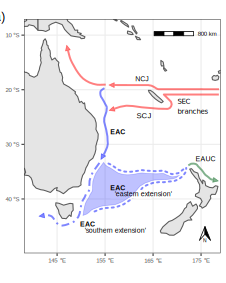
\includegraphics[width=1\linewidth]{../EDA/Fig1-study-area-raw-counts} 

}

\caption{ }\label{fig:fig1-study-area}
\end{figure}

\end{landscape}

\newpage

\begin{figure}

{\centering \includegraphics[width=1\linewidth]{../results/Fig4_partial-plots-spring} 

}

\caption{ }\label{fig:fig2-partial-plots}
\end{figure}

\newpage

\begin{figure}

{\centering \includegraphics[width=1.1\linewidth]{../results/Fig2_point-predictions} 

}

\caption{ }\label{fig:fig3-point-pred}
\end{figure}

\newpage

\begin{landscape}

\begin{figure}

{\centering \includegraphics[width=1.1\linewidth]{../results/Fig3_probability-maps-spring} 

}

\caption{ }\label{fig:fig4-prob-maps}
\end{figure}

\newpage

\begin{figure}

{\centering \includegraphics[width=1\linewidth]{../results/Fig5_spp-profiles-spring} 

}

\caption{ }\label{fig:fig5-spp-profiles}
\end{figure}

\end{landscape}

\bibliographystyle{unsrt}
\bibliography{../references.bib}


\end{document}
